\documentclass[10pt]{article}
\usepackage{graphicx}
\usepackage{pdfpages}
\usepackage{float}
\usepackage{hyperref}
\usepackage{ amssymb }
\usepackage{multirow}
\usepackage{enumitem}
\usepackage{url}
\usepackage{footmisc}
\usepackage{listings}
\usepackage{caption}
\usepackage{tabularx,ragged2e}

\captionsetup[figure]{labelfont=bf}
\captionsetup[table]{labelfont=bf}
\newlist{A}{enumerate}{1}
\setlist[A]{label=\textbf{A\arabic*}}
\newlist{B}{enumerate}{1}
\setlist[B]{label=\textbf{B\arabic*}}
\newlist{C}{enumerate}{1}
\setlist[C]{label=\textbf{C\arabic*}}
\newlist{D}{enumerate}{1}
\setlist[D]{label=\textbf{D\arabic*}}
\let\subsectionautorefname\sectionautorefname
\let\subsubsectionautorefname\sectionautorefname


%opening

\begin{document}
\begin{titlepage}
	\centering
	This present work was submitted to the institute\\
	{\scshape\LARGE i5 Information Systems \par
	RWTH Aachen\par}
	\vspace{1cm}

	\vspace{1.5cm}
	{\huge\bfseries Developing a machine-actionable process model for ethical approval workflows\par}
			\vspace{0.5cm}
Master Thesis\\
	\vspace{2cm}
	presented by \\
	{\Large\itshape Verena Schwaiger\par}
		\vspace{0.5cm}

	Matriculation Number\\
	329517
\begin{flushleft}


	\vfill
		\vspace{0.5cm}

	{\Large
	Supervisors}\\
					\vspace{0.25cm}
					 Prof. Dr. Stefan Decker \\
					 PD Dr. rer. nat. Dipl.-Phys. Cord Spreckelsen

	\vspace{0.5cm}

	{\Large Advisors}\\
	\vspace{0.25cm}
	Dr. Oya Deniz Beyan \\
	
Daniel Mietchen, Ph.D.
\end{flushleft}
				\vspace{0.25cm}


	
	

	\vfill

% Bottom of the page
	{\large Aachen, \today\par}
\end{titlepage}

%\maketitle
\newpage

 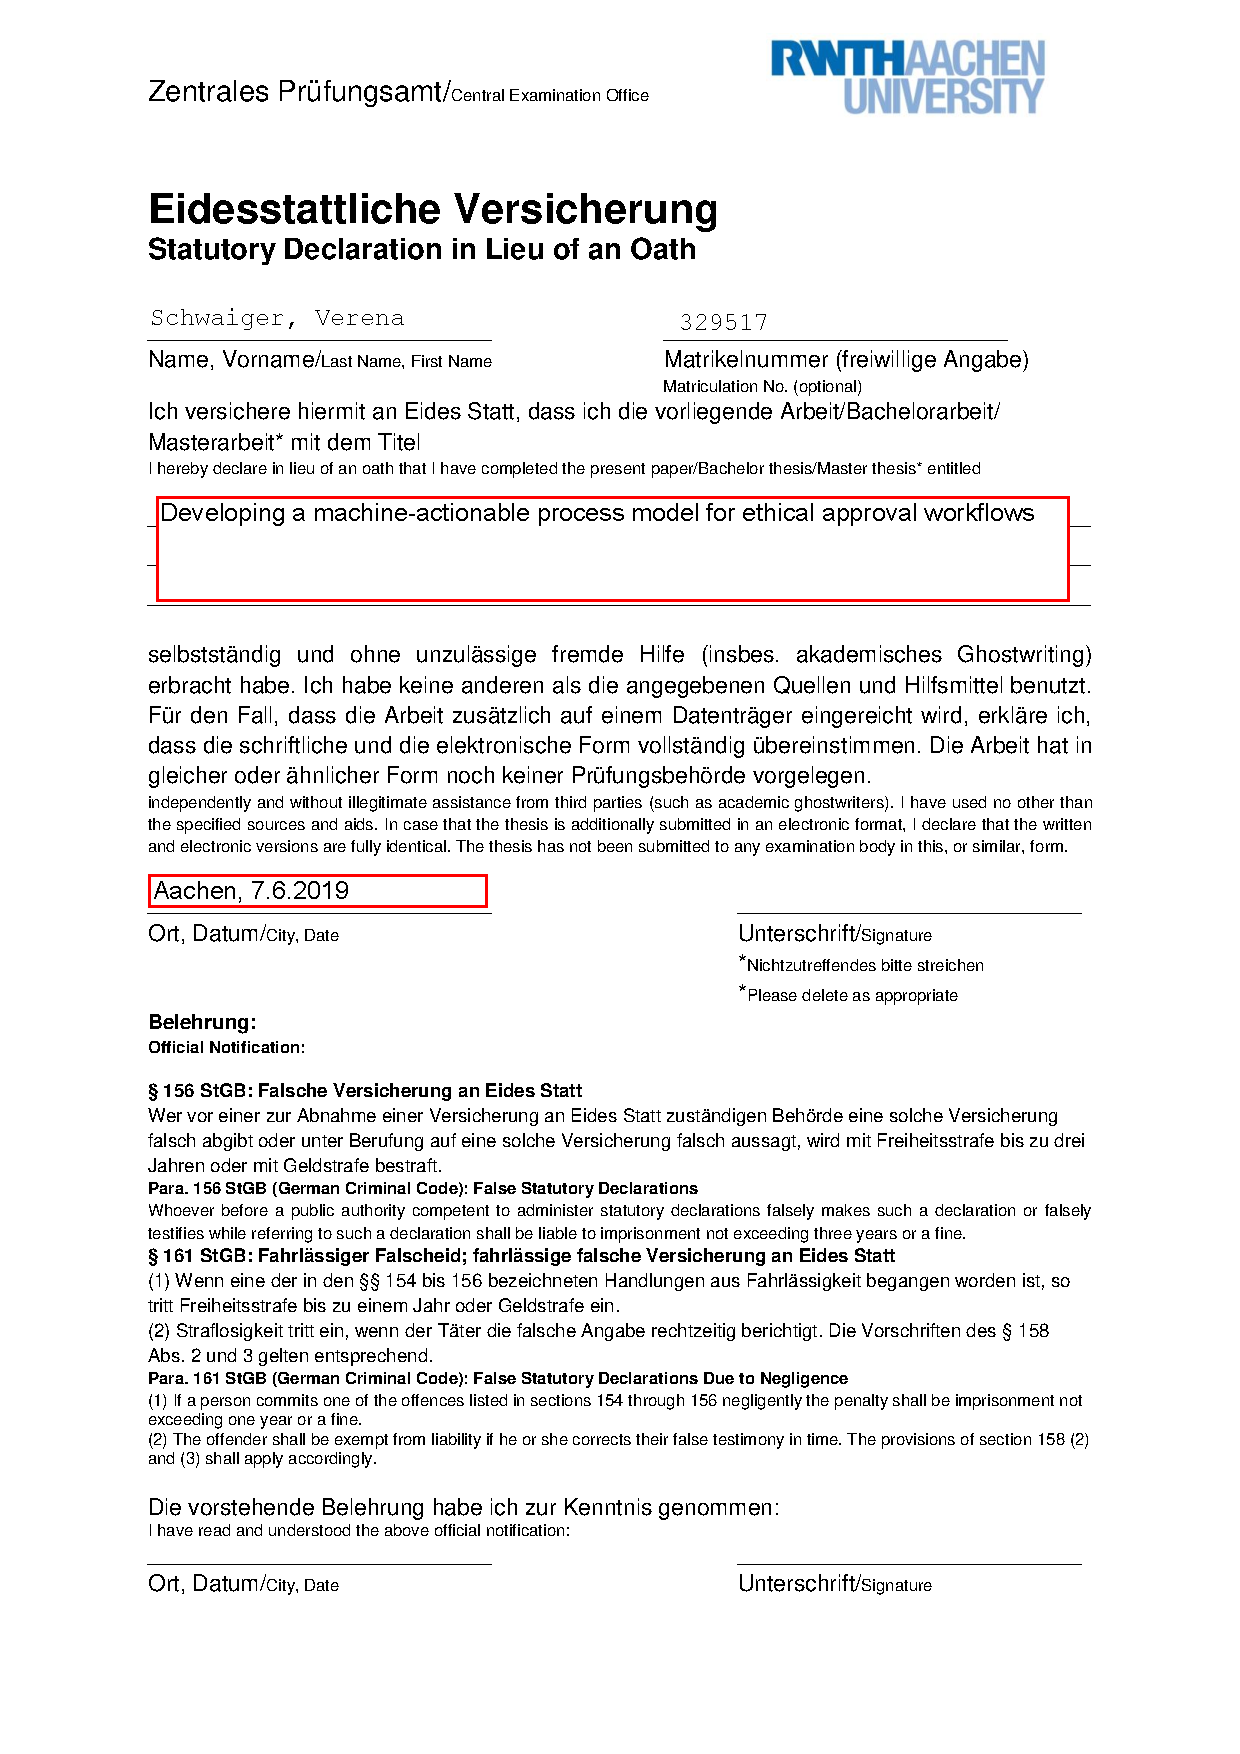
\includepdf{erklarung.pdf}
 
 \newpage
 \section*{Abstract}
 
Researchers from many disciplines have to go through an ethics approval process if their research subject meets certain criteria. 
Although the process is generally similar across institutions and fields, and in many cases governed by policies, laws or other regulations, some disciplines require different documents and steps than others and it may not always be clear which ethical body is responsible and which forms must be submitted by a researcher. 

There is currently no openly available database for previous ethics approval cases. Researchers also cannot search for approved (or rejected) studies. Many ethics committees do keep internal records and assign process numbers, which can sometimes be found listed in published studies, but these are not routinely made public. 

We analyzed the ethics approval process and formalize the collected information with a pattern language and an ontology. With these structures, we implemented a tool that aims to make ethics approval process findable, accessible and reusable under the principles for \textit{FAIR}ness and machine-actionable data management plans. An integration into the workflows of ethics review stakeholders could improve communication, research and administration related to ethics review process data.
 
 \newpage
\tableofcontents
\newpage


\section{Introduction}
\label{sec:introduction}
\subsection{Introduction to the topic}

Researchers from many disciplines have to go through an ethics approval process if their research subject meets certain criteria. 
Although the process is generally similar across institutions and fields, and in many cases governed by policies, laws or other regulations, some disciplines require different documents and steps than others and it may not always be clear which ethical body is responsible and which forms must be submitted by a researcher. This is mainly the case when a study covers multiple fields, or when researchers, subjects or study personnel from multiple institutions or jurisdictions are involved. A special case in ethics approval is secondary research. Study designs, consent forms or other data could be reusable for studies that are based on existing research. Researchers may need this data for their ethics approval application, or they may want to look into the study development and how the ethics approval process was conducted.
There is currently no openly available database for previous ethics approval cases. Although applicants have to list details of the study they would like to reuse, they do not have access to information on how the approval process for that original study went. Researchers also cannot search for approved (or rejected) studies. Many ethics committees do keep internal records and assign process numbers, which can sometimes be found listed in published studies, but these are not routinely made public. If a study has been rejected by a committee, the applicants can make changes and apply again. The more communication and reapplications happen between committee and applicant, the more complicated it gets to keep track of the already submitted documents, changes and the communication itself. Apart from the study design itself, researchers need to provide information on their data storage and sponsors, which can both have an impact on the committee's decision. 
\\

There is only few public data related to ethics approval. A study on ethnic policies in Latin America has made parts of their data publicly available. \cite{casestudy} This includes metadata, a consent form and the approval letter from their ethics review board. Through the contents of these files, the study's ethics review process has gained transparency. Anyone who is interested in the conditions under which approval has been granted can easily access them. Secondary research has access to the consent form immediately and can provide this as additional information in case they want to reuse interview data from the original study. Through metadata and DOIs, the data is searchable and available for machine consumption. 
\\

Although researchers could gain insight into how ethics approval processes are conducted  through publicly available data, not all their questions may be answered by that information. As an exaggerated example, if a research team wants to conduct a study on the impact of hot air balloons on bird migration routes, there may not be enough information available about how they should prepare for ethics review. They would have to identify potential ethical issues such as observation on private property, whether their research itself would impact bird routes or the environment, etc. This can lead to administrative problems that can delay the study timeline, if the research team does not hand in the required documents or their ethical considerations are not sufficient for the review board.\\

The ethical approval process covers a number of very different scenarios for research studies in many areas, for example the difference between vertebrates and non-vertebrates in animal studies, or the difference between conducting a field study in a dangerous or unproblematic environment. A preliminary search through published studies that have received ethics approval reveals such cases and institution-specific ethics processes. Each scenario comes with different requirements, roadblocks and forms. The forms that have to be filled out by applicants are not standardized but typically include detailed questions on the study design, including different interview and consent types as well as sections that aim to identify potentially problematic aspects (e.g. involving minors or prisoners). 
\\

In their current state, ethics approval application workflows are altogether not as transparent and integrated with the other aspects of data management as they could be. Information that has already been submitted elsewhere, for example for funding, is not commonly automatically added to applications. Data submitted to ethics committees is in general not reusable and discoverable by outsiders. Some committees still rely on paper storage. Adding machine-actionability to the process could improve these aspects and make data organization easier. As there have only been limited efforts for the automation of ethical issues and no complete solutions to these problems exist so far, there is still a lot that could be done. Since recent developments in the field are realizing a more open and accessible way of data management, a solution that aims to improve transparency for ethics fits well within current research.


\subsection{Task and goals}

Our first goal is to model the ethics approval process so that such a formalization can be reused for implementations and other work. An ontology that covers the approval process will be designed to represent the process and its data objects, their relations and attributes. With this ontology, we will have a controlled vocabulary that can be used to add machine-actionability to the storing and retrieving of ethics data. In addition to this ontology, we will describe a pattern language that formalizes problems and solutions to problems in the given domain. 

We will derive formalization and concepts from existing approval processes and experience reports. This requires a thorough research of the approval process at various institutions and research fields. Therefore, one of our tasks is to analyze the process in detail and summarize our findings.\\

To help researchers handle the approval process, a tool that automates some of the steps could be helpful. The question and goal here is to identify those steps that could be automated. Potential parts could be the identification of keywords that signal the need for ethics approval from abstracts and other available resources as gathered during the analysis phase. 

Other potential sub-tasks are the selection of stations and paths in the approval process relevant to a study and the instantiation of the correct path for each individual study. 

An important goal of our work is to make the ethics approval process machine-actionable. We will discuss guiding principles from previous work and aim to use suitable guidelines as a way to evaluate our progress. A focus will be on reusability and findability of data created during the application process. In order to fulfill this goal and further structure the approval process, permanent identifiers (PIDs) will be introduced to different documents and parts of the process.


\newpage

\section{Background}
\label{sec:background}
In this section we will give background information related to our topic. As we work with machine-actionable data management plans, we will go into how they can be beneficial to stakeholders of data management related to studies and research. A focus is on what can make data management plans machine-actionable. The concept of \textit{FAIRness} for scientific data management is related and will also be discussed. Finally, we will look at related work in the field of data management plans and ethics approval.

\subsection{FAIR principles}
With the amount of scientific data rising, searching and managing these large quantities of data becomes a challenge. In order to improve the discovery of data for researchers, publishers and anyone who wishes to reuse existing data, the \textit{FAIR} principles were introduced in \cite{fair}. \textit{FAIR} was there used as an acronym for "Findability, Accessibility, Interoperability, and Reusability". These four core principles are further broken down into multiple guiding principles. They include the use of metadata, permanent identifiers (PIDs) and indexing to improve findability and reusability. Data is defined as sufficiently accessible if common protocols are involved and if metadata is still available even after the original data has vanished. Through referencing and appropriate knowledge representation data can be made interoperable. 

As there is currently no established structure for ethics-related data that fulfills these principles, finding and reusing this data is harder than it could be.  

\subsection{Machine-actionable Data Management Plans}
Data management plans (abbreviated in the following as DMPs) have originally been designed as manually written plans for research projects that include information on different subjects relevant to the project's details and its data. Researchers use them to describe how they collect, share, archive and store data. They include information on ethics and legal considerations and the cost involved with the study (e.g. data storage). As they are created once as a text file, it is easy to set the document aside and never update it again, although the project details might change during the course of the research. (cf. \cite{madmp}, \cite{dmp})

More recently, DMPs have been created in better accordance with the aforementioned \textit{FAIR} principles. Machine-actionable DMPs are a recent development that aims to add automation and dynamic features to the original, simpler DMPs. 
\begin{figure}
\centering
	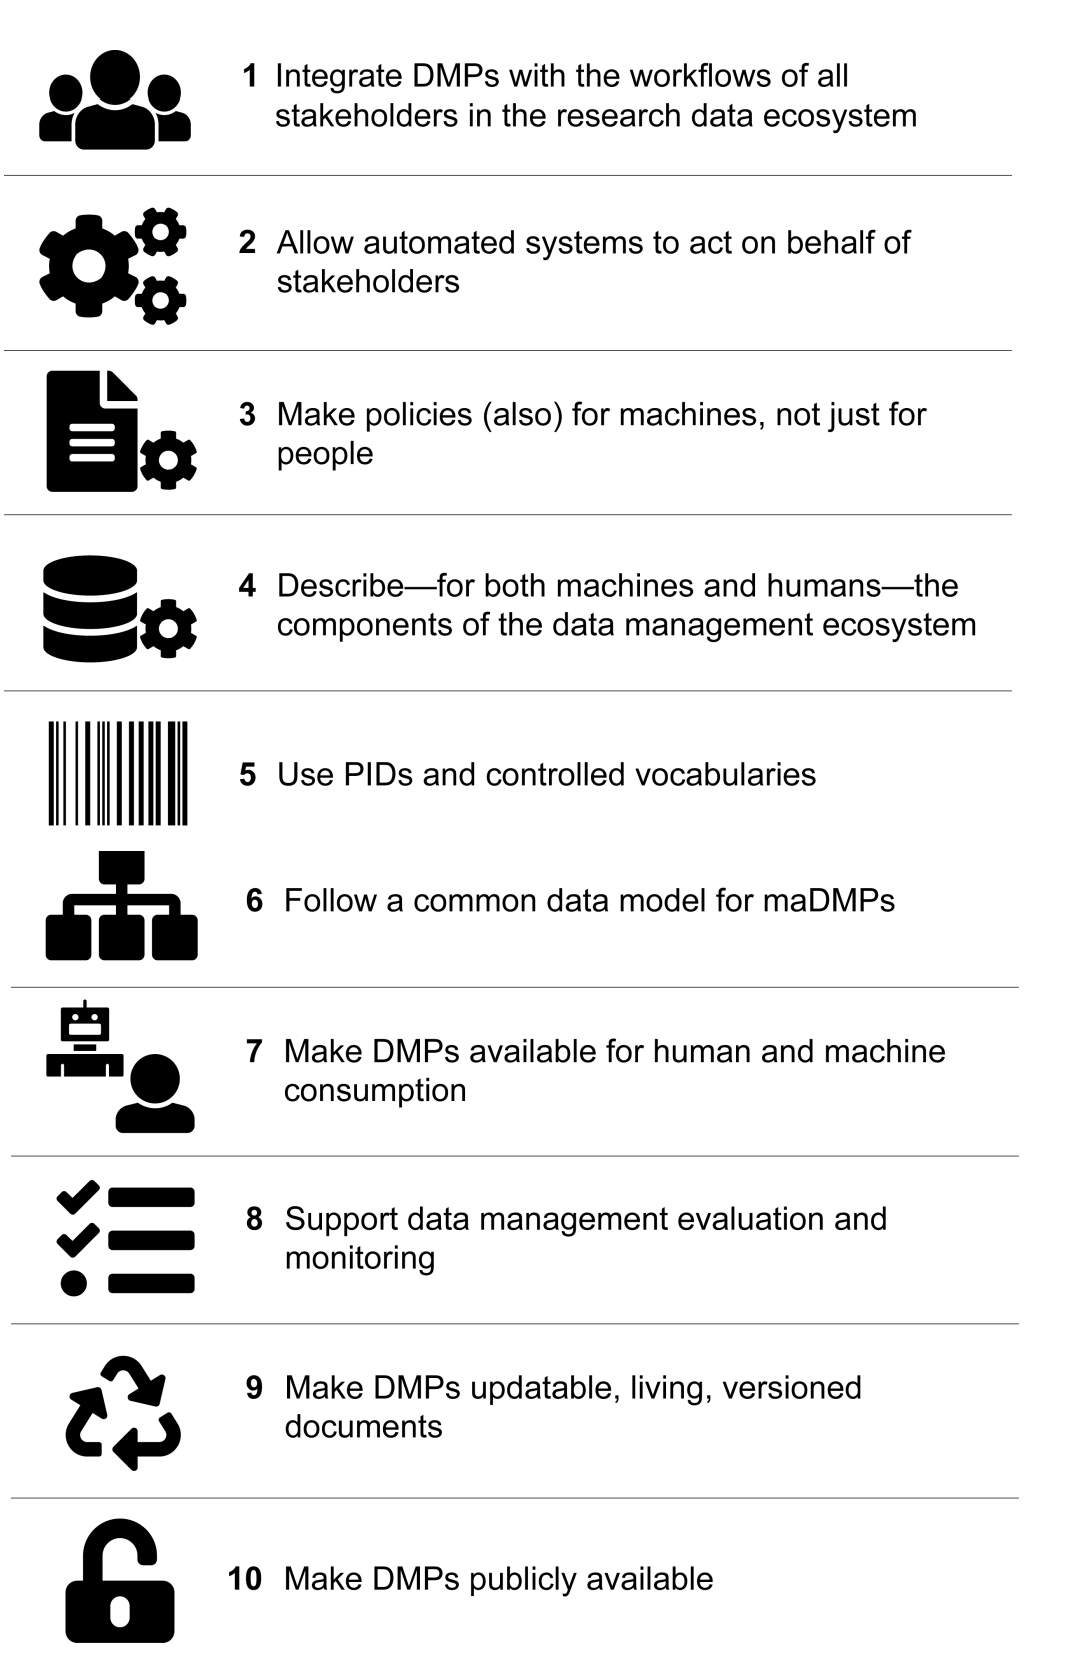
\includegraphics[width=0.75\textwidth]{img/madmpall.jpg}
	\caption{Principles for machine-actionable data management plans \cite{madmp}}
	\label{fig:madmp}
\end{figure}
As listed in Figure \ref{fig:madmp}, principles for machine-actionable DMPs concern the machine-readability and machine-compatibility. According to \cite{madmp}, all principles should be met by a data management plan, although they do not have to be implemented for all stakeholders at once. From these rules, it becomes apparent that an important part for machine-actionable DMPs is adding machine-readability by using structured vocabularies and persistent identifiers, which make data reusable and findable (principle 5). Additionally, principle 9 and 10 address the problem of static plans that are stored somewhere where not everyone can find or discover them.\\






\subsection{Related work}
Machine-actionability for DMPs has already been made possible in many aspects by the \textit{DMPTool} \cite{dmptool} and \textit{DMPRoadmap} \cite{dmprmap} projects. \textit{DMPTool} is at the time of writing used by around 40000 users with 249 participating institutions, which shows that machine-actionable DMPs have been received well. Previous efforts in these two applications include a way to automatically create a data management plan with the help of a wizard. An investigation into how parts of DMPs could be automated in the form of smaller projects has been summarized in \cite{dmpblog}. Many of these automation projects include the import of external data as a way to collect information on licenses and study details and provide an estimation of data storage costs. \\

A tool to create ethics checklists for data scientists, \textit{deon} \cite{deon}, provides the user with potential issues that need to be addressed when dealing with sensitive data especially. This includes questions on whether informed consent has been acquire from participants, how data is stored and whether the data has been analyzed sensibly. These questions have been collected by the authors from articles on data ethics and include a list of real world examples that have failed to conduct ethically sound studies. As \textit{deon} was designed as a flexible checklist, users can add or remove questions if they are not applicable to them. This idea of a checklist to help data scientists can be applied to researchers going through the ethics approval process as well. \\

Missing from these tools is an attempt to add automation to the ethics approval process itself, and in extension the documentation of ethics in data management plans. At the moment there is no concrete implementation of the idea of making the ethics process machine-actionable.

\subsection{Constraints}
We face several constraints when it comes to realizing a machine-actionable process model for ethics approval workflows. Ethical issues are not always immediately obvious. There are many nuances to consider, especially in uncommon study topics. Furthermore, ethics committees may not be receptive when it comes to making ethics processes public and transparent. The current system is often closed off and private. 
These are issues that need to be addressed further and extensively. We will provide more details on how they complicate an automation of the process in Chapter \ref{sec:analysis}.

\subsection{Summary}
We have looked into the background of machine-actionability and recent efforts to improve data management. Important for us is the goal of making data findable and reusable, as this does not apply to ethics approval-related data at this moment. Ideas from the \textit{FAIR} principles and the 10 guiding principles for machine-actionable data management plans are applicable to our scenario. With this background, we can construct a solution that addresses the problems faced by researchers who want to look further into ethics-related documents and other metadata.

\newpage

\section{Analysis of the ethical approval process}
\label{sec:analysis}
Before we could design the formal model of ethical approval processes, we first analysed the process. For this, we researched existing process guidelines and application forms. In a second research phase we collected additional information through experience reports and publications about the approval process. The knowledge gathered from both research phases is the basis for our formal concept and helped shape the concept implementation.

In this section, we describe our research approach and the collected information. We start with an overview of the approval process as derived from our research and go into the nuances of the process with a summary of experience reports.

\begin{figure}
	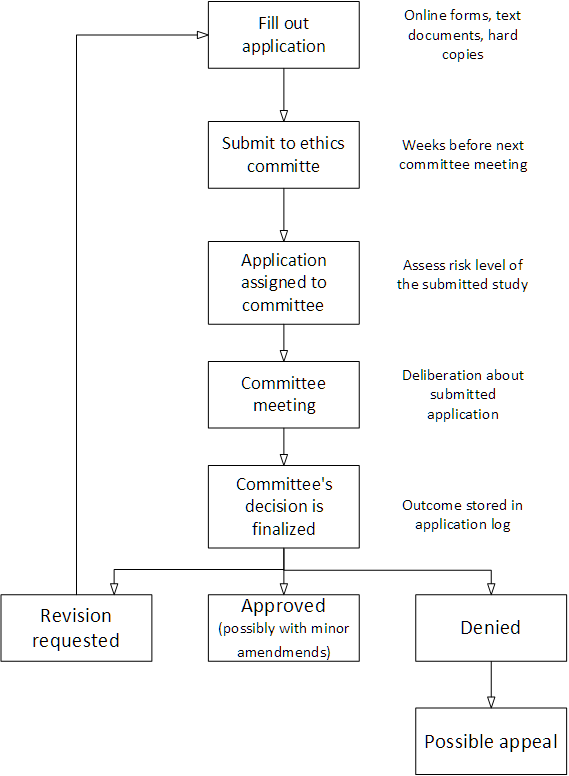
\includegraphics[width=1\textwidth]{img/process.png}
	\caption{Key steps in the ethical review process for planne studies.}
	\label{flowapplication}
\end{figure}	

\begin{figure}
\centering
	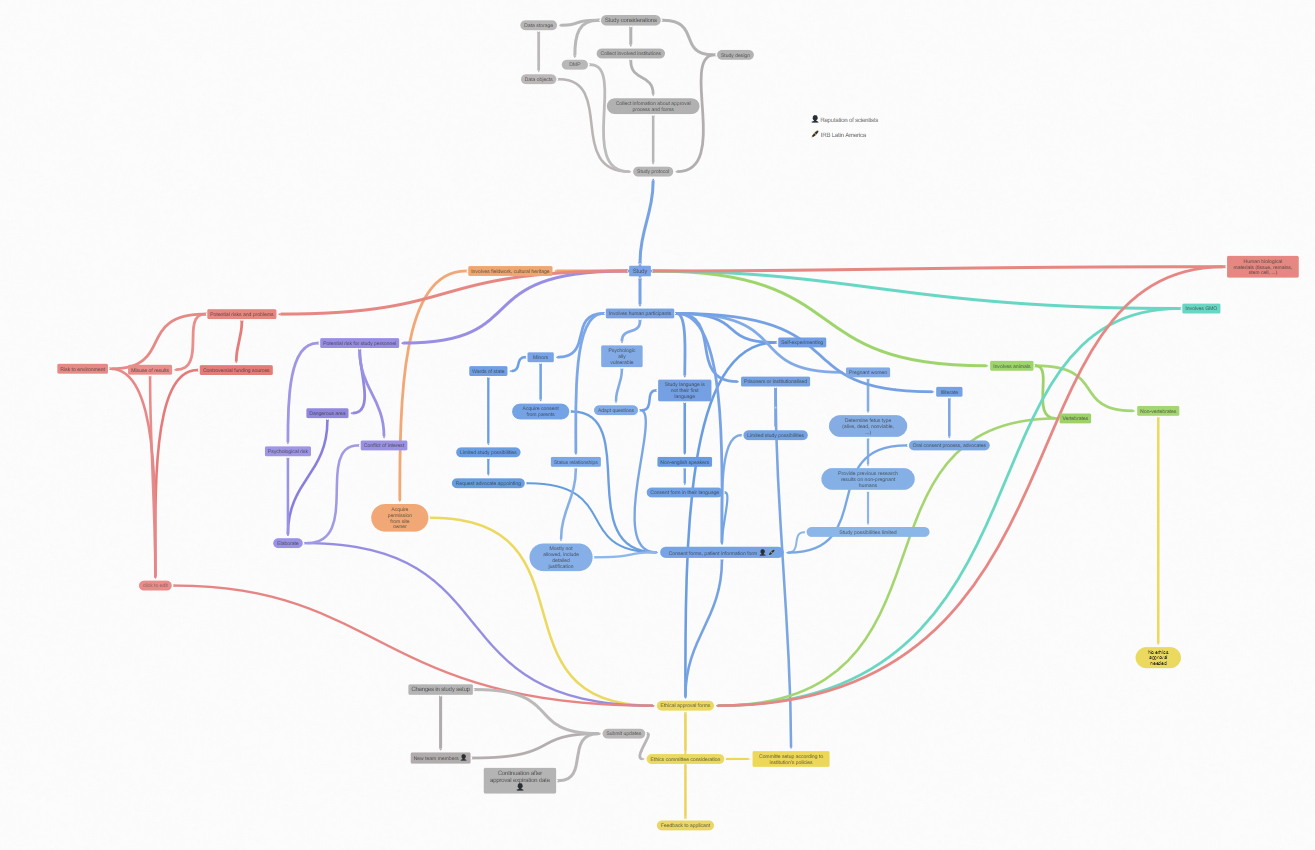
\includegraphics[width=1\textwidth]{img/processflow.jpg}
	\caption{Illustration of the large number of special cases and diverging paths that each come with different requirements.}
	\label{somanypaths}
\end{figure}	
\begin{figure}
\centering
	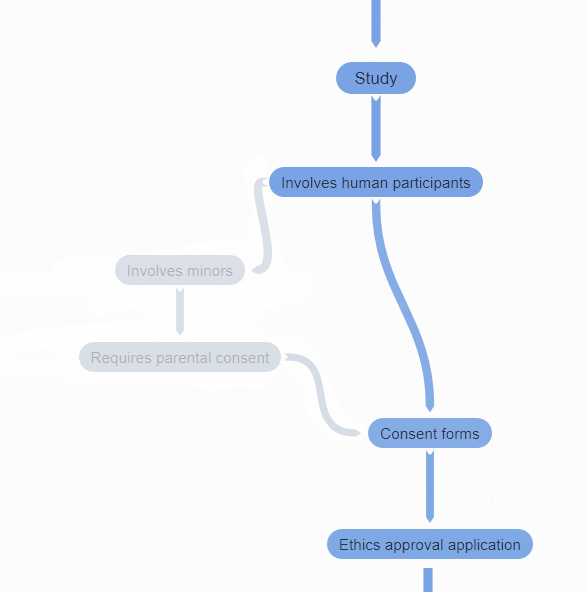
\includegraphics[width=1\textwidth]{img/processflowhlite.jpg}
	\caption{Zooming in on Figure \ref{somanypaths}.}
	\label{fewerpaths}
\end{figure}
\subsection{Process and structure}
In our first research phase, we accessed the websites of 20 ethics committees of different universities and countries of origin. Our focus was on finding out about the general application process and collecting forms and application requirements that we could use later to develop our concept model. Although specifics and application forms varied, the general structure stayed the same. Figure \ref{flowapplication} shows the application process. After filling out and submitting the application form, study authors need to wait for the ethics committee's next meeting. Depending on a first risk assessment, the applications will be assigned to a number of committee members. The committee then can reject or approve the application. Requests for revisions are possible, as well as appeals if a study has been rejected and the applicants disagree with the decision. Committees store application data in internal logs or private databases. Figure \ref{pidsnow} demonstrates how application data is stored with a PID. This PID is assigned to each application and is used internally to reference studies. This data is not accessible for outsiders, which means that secondary research and background information for published studies is limited to what the original researchers provide when contacted directly. Approvals usually expire after a certain amount of time, which varies from institution to institution.\\

After determining the common application process, we collected study scenarios from the ethics committee guidelines available to us. Many of the committees listed a number of possible signs that would lead to the requirement of an ethics application and could make an approval less likely. With these specific triggers, we can identify which studies need greater care with regards to ethical considerations. These include, for instance:

\begin{itemize}
\item Human participants
\item Human tissue or remains
\item Identifying data
\item Surveillance
\item Vertebrate animals and cephalopods
\item Genetically modified organisms
\item Stem cell research
\item Material from monuments or fieldwork on sites that require permission
\item Collected data from software usage
\item Risk to the environment
\item Risk to the research team (psychological or through work in dangerous areas)
\item Results could be misused for military or terrorist purposes
\item Conflict of interest
\item Controversial funding sources
\end{itemize}

Additionally, subgroups of these categories, for example children or prisoners, come with further restrictions and requirements.

We can then classify our collected categories into two groups: triggers that are either easy or hard to identify. The easily identifiable signs, e.g.\ as to whether human subjects are involved or not, can generally be extracted from a study summary and keywords alone. 
The ones that are harder to identify are based on context knowledge. We cannot necessarily tell, for instance, whether a study would bring risk to the environment or the involved researchers without access to the full study design and set-up. The hardest to identify are conflict of interest for researchers, which can depend on many factors, and controversial funding sources, which could be up for individual interpretation. \\

With this information, we designed a subway diagram that shows the different stations and decision points for studies. Figure \ref{somanypaths} gives an overview of this diagram. Here, we combined the process flow with decision points that determine the appropriate workflow. Figure \ref{fewerpaths} shows a close-up of one decision point. Here, our path depends on whether our study involving human participants also involves minors. As studies with minors require parental consent, the ethics approval application would have to come with another consent form. 



\subsection{Examples and experience reports}
After we analysed the general approval process as far as formalities go, we researched experience reports from the applicant's side. At first we queried existing studies on \textit{PubMed Central}. We were looking for mentions of ethics processes and PIDs with the help of regex queries. Few studies actually listed their ethics approval PID. At most, the institution where approval was granted was listed. Searching for the listed PIDs did not lead to any new information on the process for these studies. From the point of view of someone interested in the potential ethical issues of a study and how they were handled by the study's team, there were no satisfactory results. 
In addition to this, the process turned out to be frustrating for study authors as well, as evident from several experience reports.

In \cite{example1}, the authors studied the application processes of all studies submitted during a 12-month time period. They found that many studies were rejected based on not only ethical problems but also formalities. Of the observed 66 studies, 6 did not hand in a consent form. Many also handed in consent forms that were not complete enough to fulfil the university's requirements for informed consent. The authors conclude that despite the university's guidelines not all researchers have in-depth knowledge of the ethical issues related to research with human subjects, which complicates the approval process. Although revisions of application data was possible, this added time and organizational effort for the affected projects. 

Apart from this general problem, other experiences concern more specific issues.  

\subsubsection*{Studies involving multiple institutions}
In \cite{rep}, a study was designed about students and their behaviour regarding their health. After gaining approval from their own institution, the research team then reached out to a number of universities for approval for involving their students in the study. 
Although the majority of institutions saw no issue with the study, others denied approval. One reason was the similarity to other studies, which leads to a need for a searchable database of ongoing approved studies. Another was that they only wanted internal researchers to work with their students. Additionally, a different committee noted that the timing of next session would not work with the authors' planned study timeline.\\

The issue of time and planning also comes up in \cite{rephospital}, a study involving hospitals and their maternity ward patients. Here, the study gained approval by the authors' own institution's ethics committee, but gaining approval from the contacted hospitals took much longer. Not all hospitals had ethics committees and not all of those that had ethics applications available offered them electronically. Of the 87 hospitals initially identified as potential partners, 4 of those that planned to offer maternity services during the study period denied the applications. The authors' main complaint about the organizational process was the lack of uniformity. Although about 27 hospitals agreed to either collaborating with other hospitals' ethics committees or accepting an existing decision of another hospital, the other 60 hospitals required the authors to go through their individual ethics application procedure. 
Further, the study subject was considered sensitive, as it involved pregnancies. Hospitals that denied the study explained that it might put stress on some women, especially when there are problems with their fetus. 
\\

Altogether, the ethics approval process can be very complex when different institutions are involved, which all have their own guidelines. Submitting and organizing application data for multiple committees is time-consuming and can throw off a study's timeline - especially when study authors have no previous experience with the process.

\subsection{Summary}
As we have learned from our analysis of the approval process, the procedure for ethics approval can be highly complicated depending on the study topics. Although ethics committees share a common workflow (cf. Figure \ref{flowapplication}), the specifics of individual applications can be hard to determine by researchers. Researchers without an understanding of ethical issues may face administrative issues and have a harder time getting their study accepted. As committees operate separately, studies conducted at multiple institutions such as hospitals or schools face additional hurdles. Not only have not all committees digitalized their application processes, but the ones that have done so only use private databases for storing the application data and associated metadata. Although not opening up all data to the public can be a reasonable choice, it should be considered that this is not recommended by the FAIR principles. 

\newpage

\section{A formal model for ethical approval workflows}
\label{sec:formalmodel}
Based on the analysis in the previous chapter, we can design a formal model for application workflows. A formal model serves as the basis for our implementation concept. It can also exist separately from our concept and be reused for other applications related to our subject.   
In order to model the process flow, we have designed a pattern language. With this pattern language, we provide possibilities for solving problems that exist in the domain of ethics approval applications. Apart from the process flow, we also have to model the data flow, which includes documents such as consent forms and the application itself. In this chapter, we will also describe an ontology that models the components of ethical approval processes. With this ontology, we provide a controlled vocabulary.

\subsection{Requirements and characteristics}
Chapter \ref{sec:background} described the necessity of and requirements for implementing machine-actionable data management plans. As defined in the principles for machine-actionable DMPs, we need to introduce machine-actionability by providing a controlled vocabulary, PIDs and machine-readability among other characteristics.
We can provide controlled vocabulary through an ontology, which we will describe in the next section. As PIDs are barely present in current ethics workflows (cf. Figure \ref{pidsnow}), we need to include them in all formalizations. Figure \ref{pidsfuture} shows where PIDs should ideally be inserted into the process. We will describe concrete solutions for this in Chapter \ref{sec:implementation}.

In addition to these, we also need to modularize the process and identify classes and properties that are relevant for us. By modeling them formally, we can reuse and refer to them later on during the implementation. It also facilitates future work on the same topic, so they should be as self-explanatory and concise as possible.
\begin{figure}
\centering
	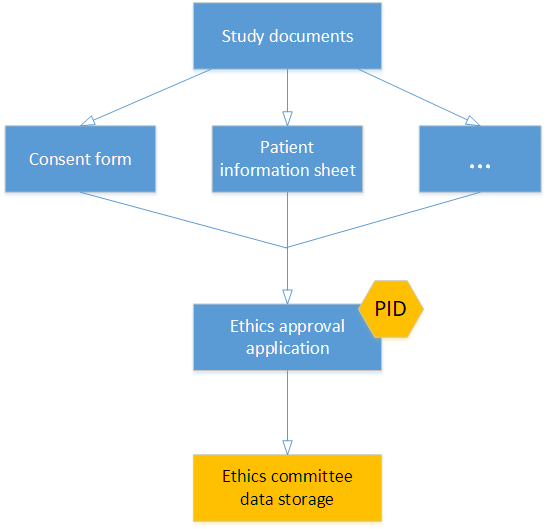
\includegraphics[width=0.75\textwidth]{img/pids_currentstate.png}
	\caption{Current state of PIDs in the ethical approval workflow.}
	\label{pidsnow}
\end{figure}	
\begin{figure}
\centering
	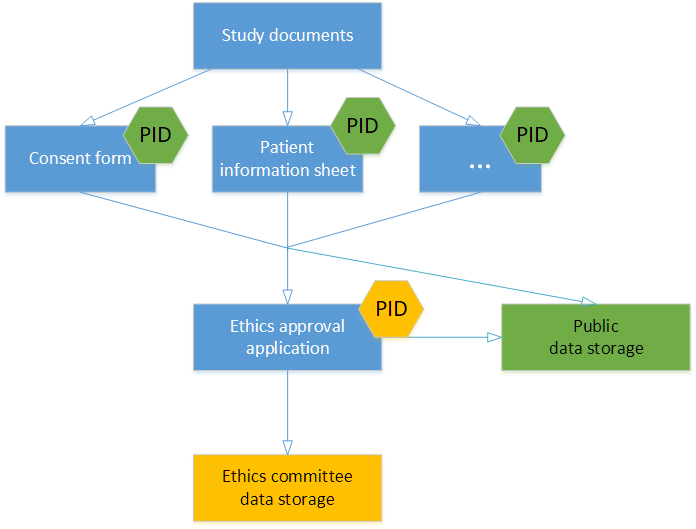
\includegraphics[width=1\textwidth]{img/pids_proposal.png}
	\caption{Concept for additional PIDs (cf. Figure \ref{pidsnow}). The committee's data store and PIDs are highlighted in yellow, our PIDs and data store are highlighted in green.}
	\label{pidsfuture}
\end{figure}


\subsection{A pattern language for the ethical approval process workflow}
 We have already illustrated the process flow in Chapter \ref{sec:analysis}, especially in Figures \ref{flowapplication} and \ref{somanypaths}. Based on our analysis of this process flow, we have designed a pattern language that we use to capture the process and its characteristics.

Originally described for the architecture domain in \cite{alexanderpatterns}, pattern languages are used to address a problem in a certain context and its solution. The author's focus was on the reusability of architectural designs. By identifying reoccurring problems, it is possible to provide solutions that can be adapted in all applicable scenarios. By splitting up a pattern language into multiple individual patterns, which can be related to each other, the author further intents to allow for variability in the pattern adaption process.

As discussed in \cite{buschmannpatterns}, pattern languages for software can be used to describe system architectures. They can be used as an abstraction of a system as well as define properties that can be used in software construction. Despite the benefits of pattern languages, the authors note that patterns can often be misunderstood. The most important clarifications for our approach to designing a pattern language are that patterns are adaptable and that diagrams that help describe a solution are not the pattern itself. This means that our pattern language will be based on our research as documented in Chapter \ref{sec:analysis}, but that not every detail may be actually present in our concept realization. 

For our pattern language, we use the structure given in \cite{patternlanguage}. The authors suggest the following layout for describing the different patterns:

\begin{enumerate}
\item Intent: A short description of the pattern idea, or goal.
\item Context: This describes the context in which the pattern becomes relevant and where it provides re-usability of the built solutions. It should be detailed enough to gain an idea about the problem space.
\item Problem: The problem that is solved by the pattern is given here. 
\item Forces: Any solution will be influenced by forces. These give information about important parts of the pattern context that are addressed by the constructed solution. 
\item Solution: By using diagrams (class diagrams, statecharts, sequence diagrams etc.), the solution is broken up into different parts. The problem is tackled from different perspectives, which is why there will usually be different diagrams. 
\item Consequences: Both the advantages and liabilities of the provided solution are discussed. 
\item Related patterns: This lists all patterns that are related or linked to each other, i.e. patterns that share elements or depend on another. This includes patterns that aim to solve conflicts that arise from the possible liabilities of a pattern's solution.
\end{enumerate}

\paragraph{Overview}
Our pattern language consists of three patterns that describe the process of applying for ethics approval. Pattern 1 is designed to describe an ethics approval instance, which includes the interactions between involved parties and the application process. Pattern 2 addresses how study details influence ethics approval and related workflows. Pattern 3 provides a solution for a problem from the previous patterns by providing a pattern to describe studies in more detail.

\paragraph{Pattern 1: Ethical approval process instance}

\begin{description}
	\item[Intent]~\par
		This pattern describes the structure of an ethics approval process instance.

	\item[Context]~\par
		A researcher is working on a study. They may have finished the full study design, know that they need ethics approval and prepared all documents and are now ready to hand in their application to their institution's ethics committee. The researcher can be part of a team or receive help from personnel from unrelated institutions. Each study is different, so the researcher has to provide enough information to the committee so that they can make an informed decision. Institutions usually have their own committees and can have multiple committees for different fields.

	\item[Problem]~\par
		A correct execution of the steps required for ethics approval is important for a successful application. We need an accurate description of the approval process that shows the involved parties, interactions and structures so that we can apply it to different situations.

	\item[Forces]~\par
	\begin{itemize}
		\item Applications may vary depending on the study type or institution
		\item For extending approval, we need a way to reference the previously handed in documents and correspondences
		\item Re-submission after rejection or a changed study set-up is possible for the applicant
		\item Committees may treat internal/external studies differently
		\item May involve multiple institutions
	\end{itemize}

	\item[Solution]~\par
		The solution is to keep progress and status of approval in a record. Additionally,  general information on institutions and applicants is stored. PIDs are created for reusability of documents and for (semi-)permanent reference.
	\begin{enumerate}
		\item The class diagram in Figure \ref{pat1cd1} shows the involved parties for one application. Each study has an application instance. Applicants are related to institutions and a research team. An ethics committee, which is part of a specific institution, processes application instances. Studies can be either internal or external. Information about the study itself as well as document details is kept for reference.

\begin{figure}[t]
\centering
	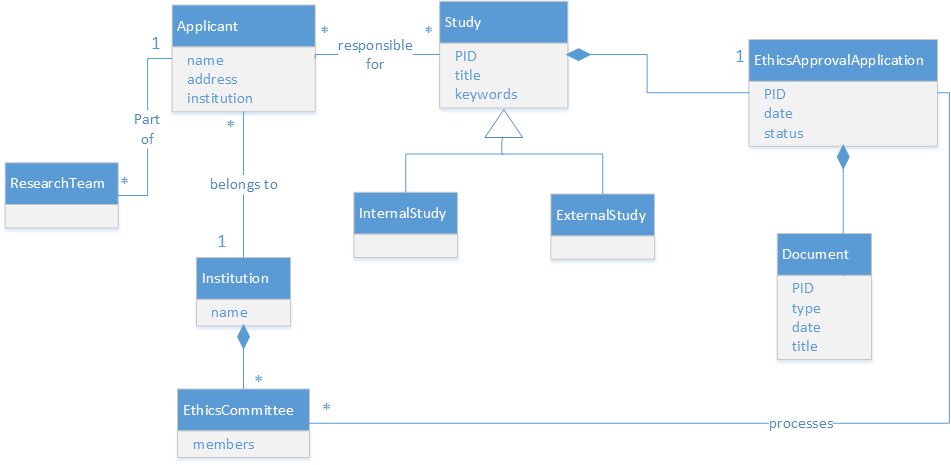
\includegraphics[width=1\textwidth]{img/involvedparties.png}
	\caption{Overview of parts of the application process.}
	\label{pat1cd1}
\end{figure}		
		
		\item The statechart in Figure \ref{pat1cd2} shows the application processing. The ethics committee starts considering the application once an application has been created and handed in. Applications can be either approved or rejected. Once closed, an application can be reopened, for example when extending the approval duration, changing parts of the study, or when applicants want to resubmit after having been rejected.
		
\begin{figure}[t]
	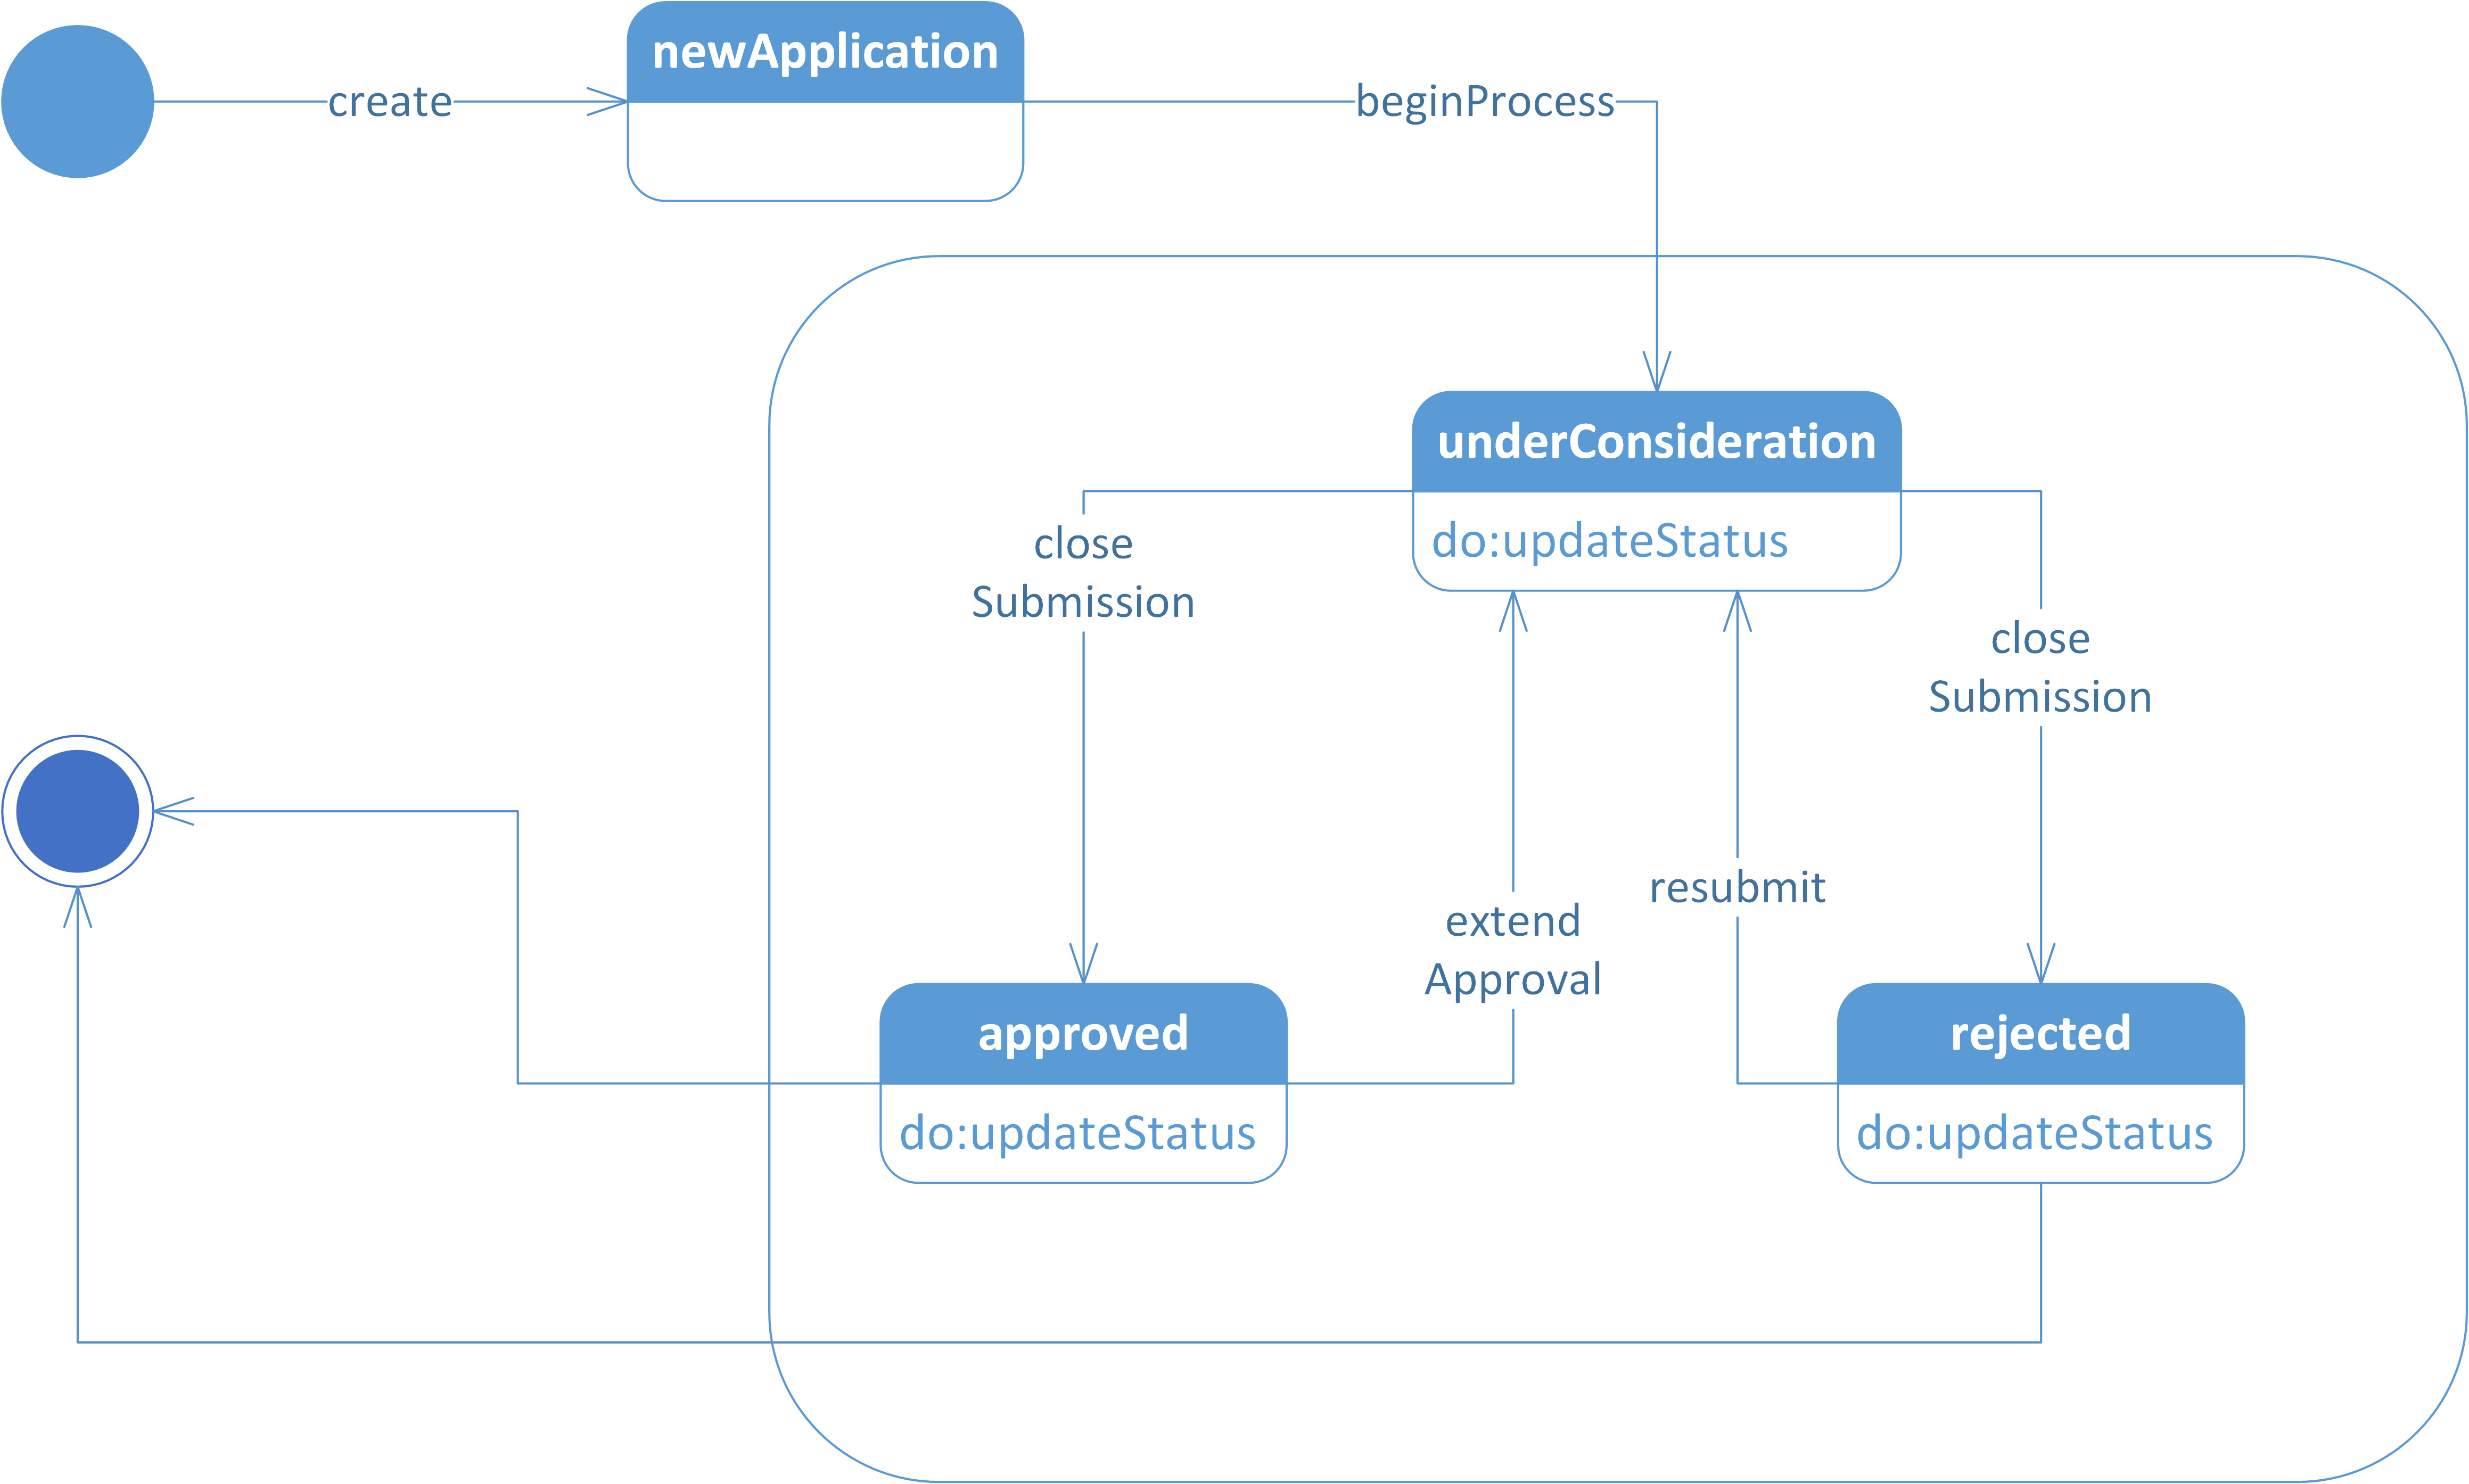
\includegraphics[width=1\textwidth]{img/approvalstate.png}
	\caption{Different states of an ethics approval application.}
	\label{pat1cd2}
\end{figure}			

	\end{enumerate}

	\item[Consequences]~\par
		\begin{enumerate}
			\item Advantages
			\begin{itemize}
				\item Application instance keeps track of status, dates and other useful information
				\item PIDs make documents referenceable for future reuse and research
				\item Applicant's and committee's institution is clear
			\end{itemize}
			\item Liabilities
			\begin{itemize}
				\item Does not detail which documents exactly are needed, as that depends on individual institutions
				\item Does not detail what may influence the committee’s decision and required documents

			\end{itemize}
		\end{enumerate}
		
		
	\item[Related patterns]~\par
		Pattern 2, pattern 3
\end{description}


\paragraph{Pattern 2: Identify a specific workflow}

\begin{description}
	\item[Intent]~\par
		Describes which components could influence the specific workflow steps.

	\item[Context]~\par
		To a researcher, it is not always clear whether their study needs ethical approval and what exactly they have to hand in. They may also be interested in finding out whether gaining ethical approval could be harder based on their study's characteristics, so that they can plan resources accordingly.

	\item[Problem]~\par
		Different studies can have different restrictions depending on their subject and/or type. It is necessary to identify these restrictions in order to correctly describe which documents the applicant has to provide.

	\item[Forces]~\par
	\begin{itemize}
		\item It is not possible to list 100\% of scenarios that lead to ethics approval requirement
		\item Different institutions have different standards and workflows
		\item Some potential triggers for the need for ethics approval can be hard to identify (e.g. potential misuse, potential psychological risk, ...)


	\end{itemize}

	\item[Solution]~\par
		The solution is to collect information on which details lead to which workflow subset.  Additional patterns are generated based on their category. Recommendations are offers and tips, not absolutes, as they may be different for separate institutions.
	\begin{enumerate}
		\item The class diagram in Figure \ref{pat2cd1} shows that every study restriction is part of an ethical concern. Ethical concerns are extracted from study details, such as study subject and type. (cf. Pattern 3 for specific description of a study)\\
		
\begin{figure}[t]
\centering
	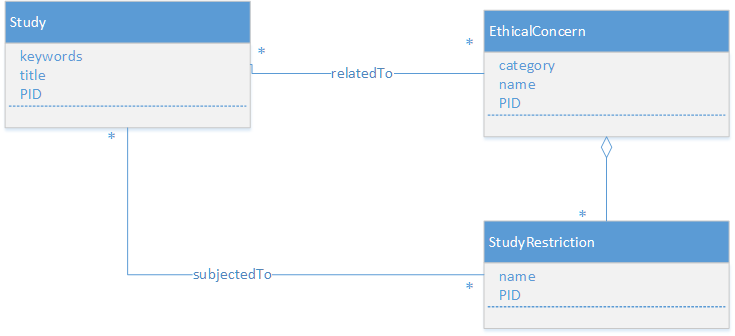
\includegraphics[width=1\textwidth]{img/identifyworkflows.png}
	\caption{Relationship between a study and its ethical concerns and restrictions.}
	\label{pat2cd1}
\end{figure}

	\end{enumerate}

	\item[Consequences]~\par
		\begin{enumerate}
			\item Advantages
			\begin{itemize}
				\item Record that restrictions come from certain ethical concerns
				\item Record categories/types/... that are used to identify possible concerns
			\end{itemize}
			\item Liabilities
			\begin{itemize}
				\item May not properly capture hard-to-identify concerns

			\end{itemize}
		\end{enumerate}
		

	\item[Related patterns]~\par
		Pattern 1, pattern 3
\end{description}

\paragraph{Pattern 3: Describe a study}

\begin{description}
	\item[Intent]~\par
		Describe the relevant components of a study.
		
	\item[Context]~\par
		 A researcher is working on a topic in a certain field. They are designing a study for their research. When using data management plans (DMPs), they will enter details about their data storage, design, research team set-up and other information that is then stored together. This information can be reused and made referenceable.


	\item[Problem]~\par
		Since the study design influences the requirements for ethics approval, we need to capture it in detail. 

	\item[Forces]~\par
	\begin{itemize}
		\item The design may change during the study
		\item The design may depend on the study topic
	\end{itemize}

	\item[Solution]~\par
		The solution is to capture the study set-up so that its components may be used to identify specific workflows.

	\begin{enumerate}
		\item The class diagram in Figure \ref{pat3cd1} shows the components of a study. The involved researchers, the study design, DMPs, data storage and data objects are linked. 
		
\begin{figure}[t]
\centering
	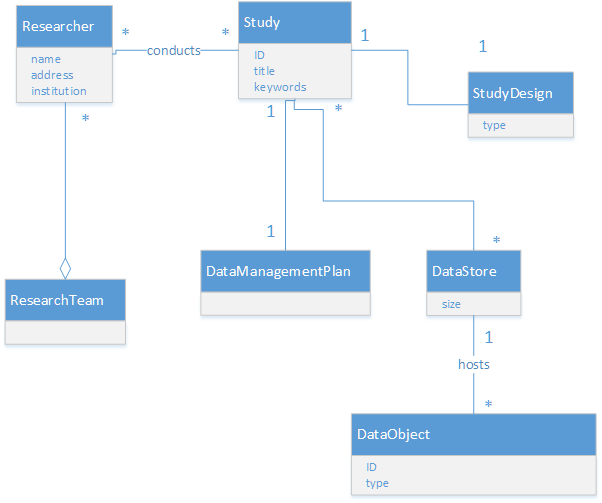
\includegraphics[width=1\textwidth]{img/decribestudy.png}
	\caption{Elements involved in describing a study and its components.}
	\label{pat3cd1}
\end{figure}	

	\end{enumerate}
	
	

	\item[Consequences]~\par
		\begin{enumerate}
			\item Advantages
			\begin{itemize}
				\item Captures components of a study
				\item Components contain important information for identifying workflows and automatization
			\end{itemize}
			\item Liabilities
			\begin{itemize}
				\item Study design, team set-up or other details may be changed during the course of the study. It would make sense to keep both old and new versions as a reference.

			\end{itemize}
		\end{enumerate}

		
	\item[Related patterns]~\par
		Pattern 1, pattern 2
\end{description}
\subsection{An ontology for the ethical approval process}
As we need a controlled vocabulary for the application procedure to fulfill the principles for machine-actionable data management plans, we designed an ontology that captures the important parts of the process and how they relate to each other. 

\subsubsection{Integration of existing ontologies}
Many of the concepts we need were already available through other ontologies, so we imported these classes and properties into a new ontology and kept references to these existing ontologies. Although most of the external ontologies that contain useful terms for us have an open license, this is not the case for SNOMED \cite{snomed} and MESH \cite{mesh}. The former must not be used in Germany, which restricts us in terms of actual reusability of our ontology. The latter has a restrictive license which requires an official application via the UMLS licensing agreement.

One of the ontologies that we incorporated, DSAP, is not available online anymore. The core concepts are still accessible via a paper in \cite{dsap}, however.

The full list of external ontologies that we can use and their licenses is as follows:

\begin{itemize}
    \item DUO - The Data Use Ontology \cite{duo} (CC BY 3.0\footnote{\url{https://creativecommons.org/licenses/by/3.0/}})
    \item ICO - Informed Consent Ontology \cite{ico} (CC BY 3.0)
    \item OCRE - Ontology of Clinical Research \cite{ocre} (no license specified)
    \item DSAP - Data Sharing Privacy Ontology \cite{dsap} (not available)
    \item AGRO - Agronomy Ontology \cite{agro} (CC BY 4.0\footnote{\url{https://creativecommons.org/licenses/by/4.0/}})
    \item SeDI - Semantic DICOM \cite{sedi} (AGPL 3.0\footnote{\url{https://opensource.org/licenses/AGPL-3.0}})
    \item IAO - Information Artifact Ontology \cite{iao} (CC BY 4.0)
    \item STY - Semantic Types Ontology \cite{sty} (CC0 1.0\footnote{\url{https://creativecommons.org/publicdomain/zero/1.0/}})
    \item NCIt - National Cancer Institute Thesaurus \cite{ncit} (CC BY 4.0)
\end{itemize}

The \textit{Creative Commons} attribution licenses \cite{cc}, abbreviated with \textit{CC BY}, allow sharing and adapting under the condition that credit is given to the original author. We fulfill this condition in our use of the mentioned ontologies by keeping concept identifiers (CUIs) and references during the import process. The \textit{Creative Commons Universal Public Domain Dedication} license (CC0) \cite{cc} allows using, distributing and modifying without restrictions.

The \textit{GNU Affero General Public License} \cite{agpl}, abbreviated as \textit{AGPL}, is a \textit{Copyleft} license. If the original ontology is used in parts in our new ontology, this requires us to grant the same, or similar, rights to distribute and modify. 

\subsubsection{Ontology design}
\begin{figure}
\centering
	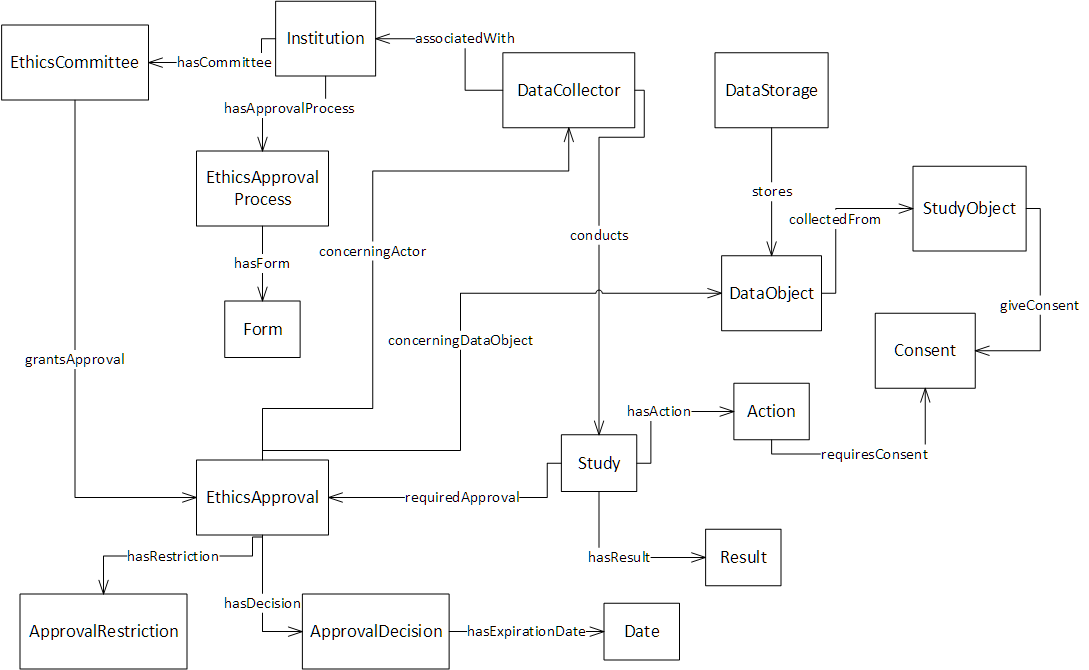
\includegraphics[width=1\textwidth]{img/ontology.png}
	\caption{Condensed overview of the ontology's classes and properties.}
	\label{ontology}
\end{figure}

An overview of the classes and properties in relation to each other is given in Figure \ref{ontology}. Our ontology is heavily based on the patterns we have designed and described in the previous section. We reused classes and properties that we introduced in the diagrams that help to demonstrate the patterns' solutions. In the illustrated ontology, the relation between ethics committee and data collectors is shown. It also describes how studies and actions related to studies are related to ethics approval. As institutions have different ethics processes, they are also integrated as their own class. The vocabulary collected in this ontology thus describes all important aspects of the ethics approval process. A full list of classes and properties (and their attribution) is available in Appendix A.


\subsection{Modelling the data flow}
Apart from the process workflow, we also have to model how documents and data are distributed between researchers, ethics committee, and other groups.
\begin{figure}
\centering
	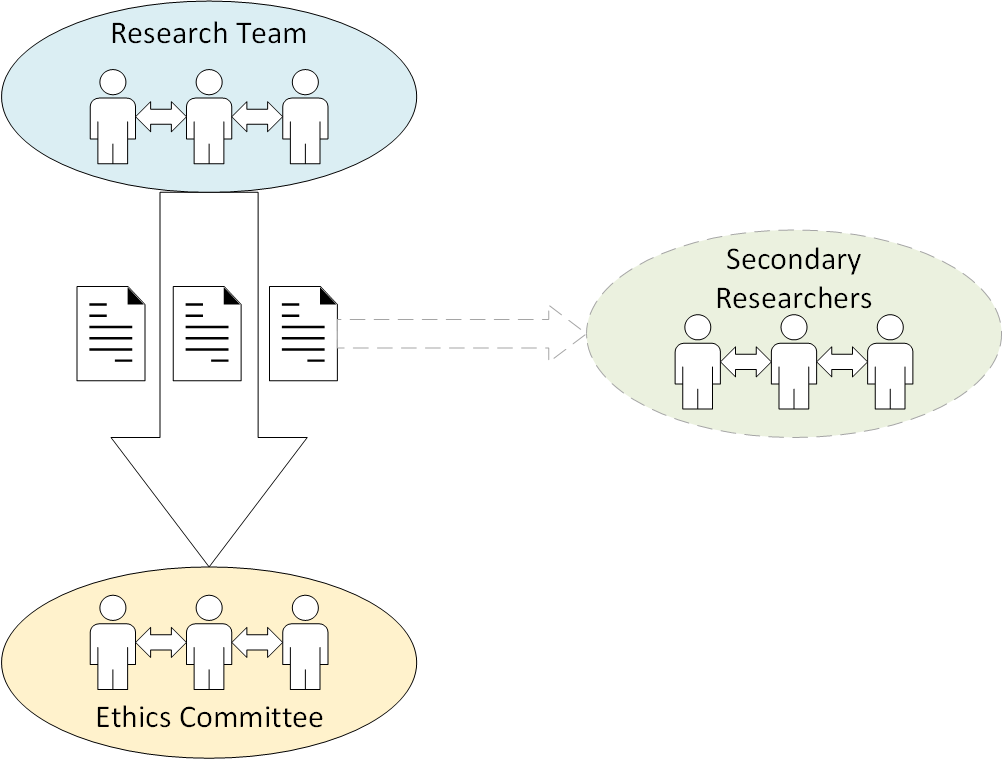
\includegraphics[width=1\textwidth]{img/dataflow.png}
	\caption{Data flow between research team, ethics committee and \-- potentially \-- secondary researchers.}
	\label{fig:dataflow}
\end{figure}

Figure \ref{fig:dataflow} shows how documents and other data are passed between different parties. In its current state, the ethics approval process has a limited data flow. Documents are passed between team members through private communication, cloud storage or similar communication solutions. When the research team submits their application, all related data and documents go directly to the ethics committee. As mentioned earlier, this may not happen digitally depending on the institution. Secondary researchers or other interested parties do not have direct access to these documents. Getting access is only possible through contacting the original research team. 

\begin{figure}
\centering
	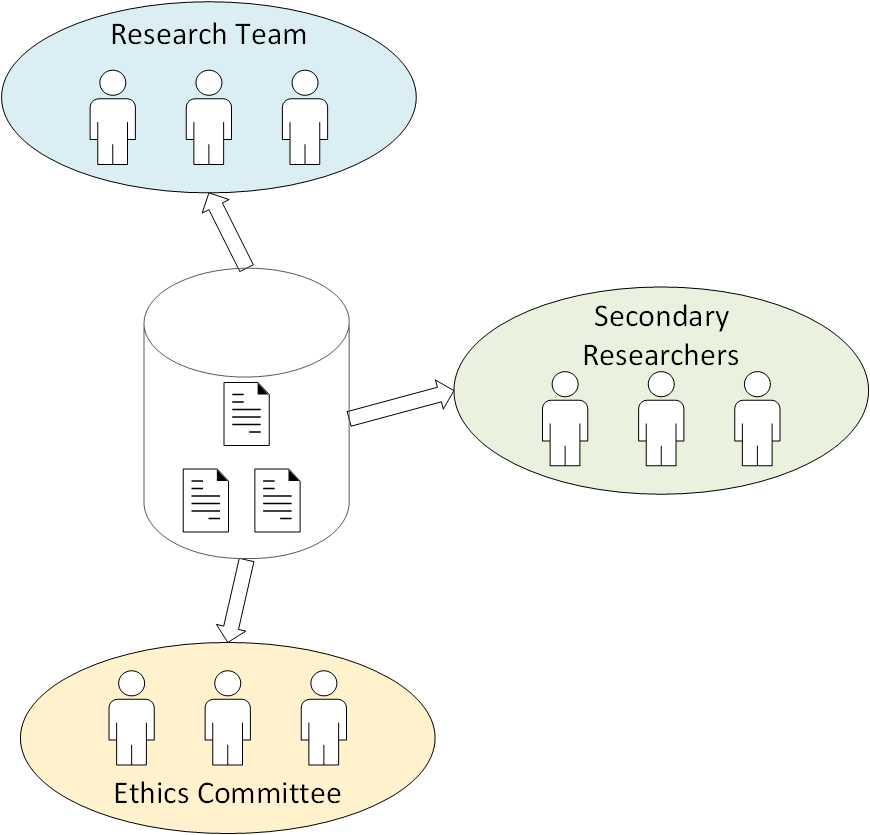
\includegraphics[width=1\textwidth]{img/dataflownew.png}
	\caption{Data flow between research team, ethics committee and  secondary researchers.}
	\label{fig:dataflownew}
\end{figure}

Figure \ref{fig:dataflow} illustrates an alternative model for the data flow. Here, documents are kept centrally. The focus of this model is the reduction of communication and increasing availability, especially internally. Each involved party has access to all data at all times. 

\subsection{Summary}
In this chapter we have documented a formal model that describes ethical approval workflows. We have designed an ontology that introduces ethics approval-specific terms and reuses relevant classes and properties from existing related ontologies. A pattern language that we designed to address problems as identified in our research was presented as an additional formalization that can be reused. Finally, we illustrated the data flow in workflows. Based on these models, we can design a concept that adds machine-actionability to the approval process.

\newpage


\section{Concept realization}
\label{sec:implementation}
This section covers our approach to realizing the model we have described in the previous section. We will first describe our concept, addressing different user needs and identifying features for our application. Then we will describe the tools and technologies used for the implementation. The implementation itself is divided into three sections: the user's interaction with a web application to determine their individual workflow, storing and managing the user-submitted data and finally giving the user feedback about their submitted data. An example walkthrough of the application and its possibilities is given afterwards. Finally, we describe our evaluation process and the results.



\subsection{Implementation concept}
As discussed in Chapter \ref{sec:analysis}, there are three main perspectives to consider when making ethics approval workflows machine-actionable: 
the perspective of those that require assistance for their applications, the perspective of those that want to research existing material and the perspective of an ethics committee. 
We will describe the requirements for both perspectives first before going into the details of how we addressed them. In the following, we will refer to the first perspective as the "author perspective" and the latter as the "research perspective". Other stakeholders according to \cite{madmp} will also be addressed.


\subsubsection*{Features}
Table \ref{tab:featuresa} shows potential features for the application from different perspectives of the stakeholders mentioned in \cite{madmp}. In the following we will discuss these features and their feasibility.

\renewcommand{\arraystretch}{2}%
\begin{table}
\centering
\begin{tabular}{|l|l|c|}
\hline
\textbf{ID} & \textbf{Feature} & \textbf{Feasibility} \\ \hline

\multicolumn{3}{|l|}{Author perspective} \\ \hline
A1      & Identify application requirements       &    $\circ$  \\ \hline
A2      &   Checklist    &   $\checkmark$   \\ \hline
A3      &    Managing application data   &   $\checkmark$   \\ \hline
A4      &   Similar studies    &   $\checkmark$   \\ \hline
A5      &   Public file storage    &   $\checkmark$   \\ \hline
A6      &   Timeline    &   $\times$   \\ \hline
A7      &   Predicting approval/rejection   &   $\times$   \\ \hline
\multicolumn{3}{|l|}{Research perspective} \\ \hline
B1      & Browse existing application data   &    $\checkmark$  \\ \hline
B2      &  Specific queries  &   $\checkmark$   \\ \hline
B3      &   Access application documents  &   $\checkmark$   \\ \hline
\multicolumn{3}{|l|}{Patient perspective} \\ \hline
C1 & Access background information on studies & $\checkmark$ \\ \hline
\multicolumn{3}{|l|}{Ethics committee perspective} \\ \hline
D1 & Access decisions of other institutions & $\checkmark$ \\ \hline
D2 & Reuse publicly available documents & $\checkmark$ \\ \hline
\end{tabular}
\caption{Overview of potential useful features and their realizability from different stakeholder perspectives.}
  \label{tab:featuresa}
\end{table}


    \begin{A}
      \item Ideally, our application can be used to find out which documents should be provided by the applicant. Although we can identify obvious requirements, such as consent forms when human participants are involved, we cannot ensure completeness. There are too many possible special cases and outliers, cf. Chapter \ref{sec:analysis}. 
      \item For self-organizational purposes, users should have a way to track their  progress on creating and publishing their application documents. Providing a checklist that shows the user their required hand-ins (forms, information sheets, ...) bases on the identified requirements can be implemented easily. The user should here be able to save their checklist progress.
      \item Users should be able to provide and manage their ethics application data on our web application. Application data provided by the user can be stored in a private database. Data in that database should not be publicly available unless the user wants it to be. The user should be able to add, edit and delete their data, which can easily be implemented. 
      \item Researchers may be interested in how the ethics approval process was done by authors of similar studies. This can also help them gauge the difficulty of gaining approval for their study. Similar studies can be shown based on a simple recommendation algorithm. As it is common for studies to have keywords in abstracts and descriptions, we can use these to find studies that share topics. 
      \item As application data has so far only been stored in private ethics committee databases, we are interested in making this data public for reusability and searchability. Although users may not want to (or have the right to) publish all their data and files, it could still be possible to at least make metadata with administrative details or other descriptive metadata accessible. Through metadata, we can then keep some record of a study and its data public even if sensitive documents could not be made public. A public storage for application files and forms can be realized with existing tools. Additionally, research support staff can immediately access documents on this database once it is uploaded. 
      \item Ethics applications depend on the schedule of ethics committee meetings. Approvals also don't last indefinitely and may need to be renewed during the course of a study. Although a timeline showing researchers their approval expiring date or their application's due date would be helpful, ethics committees do not share the same timelines and deadlines. A correct timeline would require the user to input all due dates themselves to generate countdowns, which would then still not account for changes from the committee's side. 
      \item As shown in Chapter \ref{sec:analysis}, ethics committees do not always come to the same conclusion, and decisions often hinge on fine details. Decisions can also depend on already running studies, which we do not have access to. We therefore cannot reliably predict approval or rejection. Through the public storage, we can at least provide a way to go through approved or rejected  studies for the user.
    \end{A}
    
    \begin{B}
    	\item Researchers may be interested in existing studies and their approval status as well as look for background information on the organizational ethical details of a published study. As we use a public storage in \textbf{A5}, this storage can be browsed by anyone interested in researching previous studies.
    	\item Apart from accessing certain studies or searching studies broadly, for example in categories, users may also want to use more detailed queries. Specific queries that can be executed by a user who wants to research existing materials and studies can be realized in various ways, as long as there is a query endpoint accessible by the user and the data is structured correctly.
    	\item Apart from searching for studies, users may also simply want to access application documents, for example if the public storage is used by a research team for reference on which documents are ready for submitting. As in \textbf{B1}, this is realized through \textbf{A5}.    
    \end{B}
    
    \begin{C}
        \item  Patients and study participants may be interested in learning more about the studies before or after signing up for them. Through a public data storage (cf. \textbf{A5}), they can look up additional information, which makes the studies more transparent.
    \end{C}
    
    \begin{D}
        \item As seen in the experience report in \cite{rephospital}, ethics committees may want to agree to a study once it has been approved by another institution. Keeping track of the application status and documents in a public storage (see \textbf{A5}) would make this process easier and decrease communication efforts.
        \item As studies need to be re-approved after a certain amount of time has passed and applicants can reapply for approval if they have been rejected, ethics committees need a database if they want to simplify this process. As not all committees have a digital storage set up (cf. \ref{sec:analysis}), they may want to use a publicly available database.
    \end{D}

\subsection{Tools and technologies}
In order to realize our features from Table \ref{tab:featuresa}, we researched different tools and technologies. As the DMPTool and DMPRoadmap use Ruby on Rails\footnote{\url{https://rubyonrails.org/}}, it would be beneficial to use this framework as well in order to allow for potential integration and interaction. Ruby on Rails offers several possibilities for the database we need for the web application. We decided to use a PostgreSQL database as the same configuration is used in the existing DMP tools. 

It became clear during the implementation preparations that the existing JavaScript support in the Ruby on Rails framework was too limited in terms of the reactivity that we needed to build a user-friendly interface. For that reason, we integrated Vue.js\footnote{\url{https://vuejs.org/}} for the front-end and kept Ruby on Rails as the back-end. For the communication between both, we use Axios as a promise-based HTTP client. 

Finally, we needed a publicly available, browsable database for the research perspective. For this purpose, we looked at different MediaWiki-based configurations. 

Our implementation is versioned with Zenodo\footnote{\url{https://zenodo.org/}} and available through the DOI \url{https://doi.org/10.5281/zenodo.3241002}.

\subsection{Architecture}
Figure \ref{wikibackfront} shows how the frontend, backend and the MediaWiki interact with each other. Through the frontend application, Axios requests are sent to the backend. Depending on the request, the backend API sends data to the MediaWiki, or the application's separate PostgreSQL database, or both at once. The MediaWiki will only store study data that the user wishes to make public, while the PostgreSQL database will store additional private information as well as user data and form data (such as the filled out questionnaire). Data is only retrieved from the PostgreSQL database in this setup. Data from the MediaWiki would only be retrieved through a SPARQL endpoint when an RDF store is set up for the MediaWiki. As we save all study data that is available on the wiki pages in the PostgreSQL database anyway, we do not need to use the RDF store to retrieve study data here. SPARQL queries will only become relevant when users wish to query the MediaWiki for specific studies.
\begin{figure}
	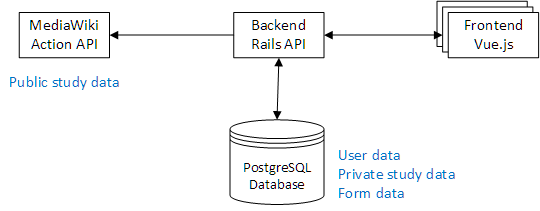
\includegraphics[width=1\textwidth]{img/wikibackfront.png}
	\caption{Overview of the interaction between frontend, backend and MediaWiki}
	\label{wikibackfront}
\end{figure}	

\subsection{Managing user workflows}
We will use the feature identification introduced in Table \ref{tab:featuresa} to go through the implementation parts related to user workflows. The user of our web application can go through the following processes:
\begin{enumerate}
\item Create a study, which is stored in a database
\item Answer a questionnaire to determine their workflow
\item Provide further study data
\item Review questionnaire
\item Use a checklist that shows documents to submit
\item Find similar studies
\item Browse and query public study data
\end{enumerate}

\subsubsection{Identify application requirements}
In order to correctly identify the requirements that would come with each individual study, we considered two possibilities early on. The first was to use a questionnaire with questions derived from the ethical approval processes of the institutions that we analyzed in the research phase. The second was to use topic mining on study abstracts or descriptions provided by the user to extract keywords for a quick categorization. 

\paragraph*{Topic extraction}
Although the second possibility would be more convenient for the user, it would be impossible to get a complete requirement list. We tried out topic mining and keyword extraction libraries such as Mallet \cite{mallet} and Smile \cite{smilekeyword} as well as basic natural language processing concepts. As an example for extracted topics, the following five topics were extracted from a randomly picked study's summary\footnote{\url{https://www.ncbi.nlm.nih.gov/pubmed/29785283/}\label{topicex}}  (sorted by topic importance as determined by Mallet):
\begin{itemize}
\item PPI (which stands for "patient and public involvement")
\item trial
\item group
\item researchers 
\item effects 
\end{itemize}

Although the topics correctly represent the study contents, we cannot confidently infer ethics requirements from them. This study selection turned out to be a good example of how context matters \--- although we know from reading the summary that the study subjects were researchers,  this would not be the case for most studies. \\

 Similarly, using natural language processing techniques such as Part-of-Speech-Tagging to remove stop-words and focus on word groups formed by adjectives and nouns also did not yield satisfying results for our scenario. \\
 
Altogether, topic extraction would only make sense for us as an additional feature, but not as a way to determine the appropriate workflow together with which documents have to be handed in by the research team.


\paragraph*{Questionnaires}
As a more precise alternative, questionnaires can be used to model a tree diagram such as the one seen earlier in Figure \ref{somanypaths}. With each question, we can determine which path the user would take. As we model the question data, we can include references to requirements and other relevant data for each question that can later be used to guide the user based on their input. 

An early concept for this questionnaire can be seen in Figure \ref{fig:questionnaire1}. As the user selects the appropriate answer, we can immediately display warnings and requirements. As long as we keep a tree structure, we can also hide questions that are irrelevant depending on the user's choices. For example, we do not need to ask the user whether their study involves vertebrate or non-vertebrate animals when we already know that there are no animals involved at all. Therefore, we decided to organize questions into categories with sub-questions. Our question tree was then derived from the ethics applications we analyzed in the research phase. The full list of questions we implemented is available in Appendix B.

\begin{figure}
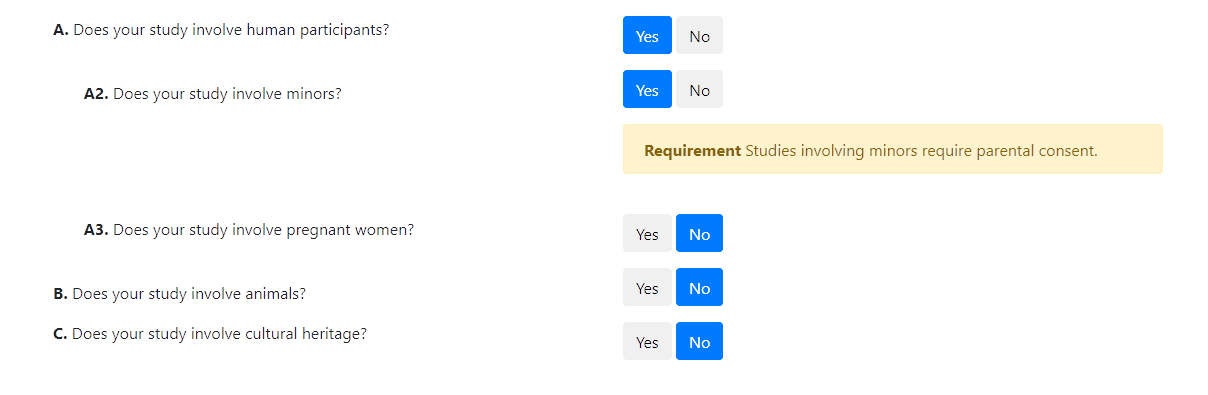
\includegraphics[width=1\textwidth]{img/questionnaire.jpg}
\caption{Early concept for a questionnaire that determines which documents and other information have to be provided by the study authors.}
\label{fig:questionnaire1}
\end{figure}

\subsubsection{Organization of questionnaire data}

After collecting the questions, we had to decide how to store them. We looked at XML, JSON and RDF as potential candidates. We will discuss the advantages and disadvantages of each language with examples. 

Each method should be capable of storing the following information for each question:
\begin{itemize}
\item PID
\item The question as a string
\item Warnings or comments
\item Requirements related to the question response (documents, forms, ...)
\item Classes (e.g. \textit{Prisoner}, as derived from our ontology)
\item A reference to its parent question
\end{itemize}

\paragraph*{XML}
XML can easily be structured as a tree. This fragment shows how instead of building nested structures, we can use values to link questions with each other. Each question is given a unique ID. We can reuse that ID for storing additional information related to each question.

\noindent

\begin{minipage}{0.97\textwidth}
\begin{lstlisting}[frame=single]
<?xml version="1.0"?>
<process>
 <decisions>
   <decision id="A" yes="A2" no="B">
     <question value="Are human participants involved?">
     </question>
   </decision>
 </decisions>
</process>
\end{lstlisting}
\end{minipage}
\paragraph*{JSON} The JSON format is also suited for a tree structure. Although we are more limited in terms of stylizing values in order to be better readable by humans, we can make use of arrays. As our application is using JavaScript, JSON has an advantage here for easier processability. This fragment shows how we can organize questions and sub-questions.

\begin{lstlisting}[frame=single]
{
  "id": "A",
  "category": "A",
  "label": "Are human participants involved?",
  "requirements": [
    (...)
   ],
  "children": [
    (...)
   ]
}
\end{lstlisting}

\paragraph*{RDF} 

Unlike XML and JSON, RDF can also build graph structures. As some process steps can have multiple predecessors, RDF would be the most suitable option for storing this type of information. We can organize the question data by using existing ontology properties, for example as follows:

\begin{lstlisting}[frame=single]
<A>
    rdfs:subPropertyOf <root> ;
    rdf:type "A" ;
    rdfs:label "Are human participants involved?" ;
    rdfs:comment "You need informed consent" .
\end{lstlisting}

\paragraph*{Conclusion}
Although we initially thought that RDF would be the ideal candidate due to the graph structure and its involvement in the Semantic Web, the integration of it into our JavsScript-based front-end application was less than ideal. As our front-end was designed to be reactive especially while filling out the user questionnaire, we had to convert the question data into JSON. Since the user's completed questionnaire is stored and later re-used to determine requirements, keeping it in one data format was preferable. During the implementation phase, the lack of a graph structure turned out to be insignificant for our purpose. Most of the potential problems, like a requirement applying to several questions or a question having multiple parents could be addressed by an informed re-structuring of the question data. \\
Even though RDF was therefore not suitable for our web application, it was still ideal for our public data storage, as we will expand on in Section \ref{sec:publicdata}.

\subsubsection{Managing application data}
As mentioned in the previous section, application data such as the completed questionnaires have to be stored in a private database so that we can reuse the data for our other features. The user should be able to edit and delete their data later on. This only applies to data stored on our application's end \-- once the user has submitted this data to the ethics committee, that data is stored on the committee's database and cannot be edited or removed by the user.

\paragraph*{Data model}

\begin{figure}
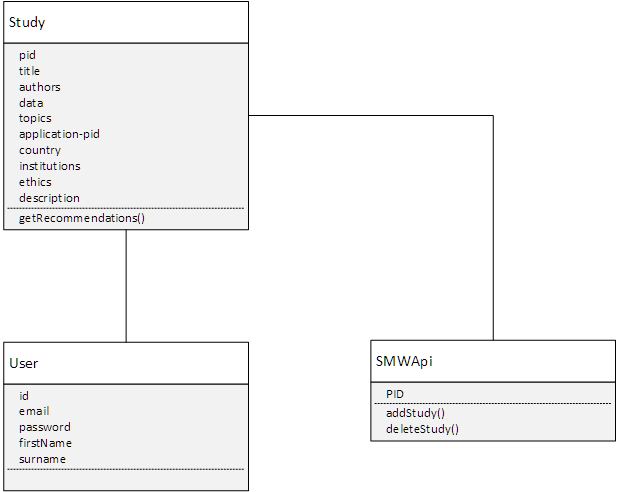
\includegraphics[width=1\textwidth]{img/classes.png}
\caption{Model used for the database scheme and helper functions. Besides the classes for study and user data, the \textit{SMWApi} class is used for communicating with the public data storage, which will be discussed later on.}
\label{fig:model}
\end{figure}

Figure \ref{fig:model} shows the entities we used together with the used attributes and helper functions. Each user-submitted study is assigned a serial ID in the PostgreSQL database. With this PID, study data is updated or deleted in the database. It serves as a unique identifier throughout the data object's life cycle. 

As we set up the back-end as an API, \texttt{POST}, \texttt{PUT} and \texttt{DELETE} requests are sent from the front-end via Axios. 

\subsubsection{Checklist}
For the checklist feature, we reused the questions in JSON format. Requirements for us are files or documents that have to be submitted together with each approval application. These requirements depend on what the user has selected in their questionnaire, so we store them alongside other question data. For each requirement that is listed in the individual questions, we track whether the user has checked the item off. On the front-end, we keep the checklist savable and updated. We also display links to a file upload form with which the user can submit documents to their study's MediaWiki page. To reduce user efforts, we automatically include information on the study ID, the type of document (consent form, info sheet, ...) and the document's automatically generated PID.

The PID we generate here is based on the study ID and a randomly picked number between 1 and 10000. It will be in the format $ID-00000$.

\subsubsection{Similar studies}
We use a simple algorithm to find similar studies. User-submitted keywords are stored in the PostgreSQL database. When the request for similar studies is sent to the back-end, we look at the intersections between the user's study and all other studies. If a study shares more than 40\% of its keywords with the user's study, it is added as a recommendation. Recommendations are then displayed as links to the MediaWiki. 
As this method performed fast, it is suitable for a quick display of potentially related studies. It also serves as a simple alternative to SPARQL queries. This features is open for future improvements, including semantic similarity, similarity between concepts in different languages, and other more advanced methods. This could be supported by controlled vocabulary through a Wiki solution with a semantic structure. 


\subsection{PIDs and data storage}
\label{sec:publicdata}
Our main concern in choosing an appropriate storage solution for user-submitted study data was the support of RDF triple integration. As one of our goals is to make study-related files such as (empty) consent forms and general study data publicly searchable and reusable, we looked at Wiki-based solutions. 

\subsubsection{Choosing the right data storage}
As there are several possibilities for setting up a MediaWiki\footnote{\url{https://www.mediawiki.org/wiki/MediaWiki}} through extensions that improve semantic searches and data storage, we first narrowed it down to the two solutions that seemed most suitable for us: 
a Wikibase-oriented setup and a Semantic MediaWiki. \\

In our first approach, we tried out Wikibase\footnote{\url{http://wikiba.se/}}, an extension for MediaWiki, as it is heavily based on storing data in a structured way. Data values are stored in the form of statements. With an RDF-oriented store, SPARQL queries can be executed on the data. Data properties are linked and can lead the user to new information. With such a setup, data entered into a MediaWiki gains semantic value instead of being only available as pure text.

The Wikidata\footnote{\url{https://www.wikidata.org/}} project uses a Wikibase installation. Figure \ref{fig:wikidata} shows how statements about a data object (in this example the data object "Earth"\footnote{\url{https://www.wikidata.org/wiki/Q2}}) are displayed on its Wikidata page. The RDF triple consists of the Wiki URL as the subject, the predicate (here "instance of" and "part of") and the object. Object values link to their data objects, if available. References can be directly inserted into this setup for each triple, which can be used for external links related to an object. 

Although a basic Wikibase extension setup would have been highly suitable for our application, querying the data via a SPARQL endpoint would only be possible using RDF database dumps. A synchronized triple store is only available through a special Docker image. As Wikibase was developed mainly for Wikidata and has a less customizable look and structure, we looked at other possibilities as well.\\ 


\begin{figure}
\centering
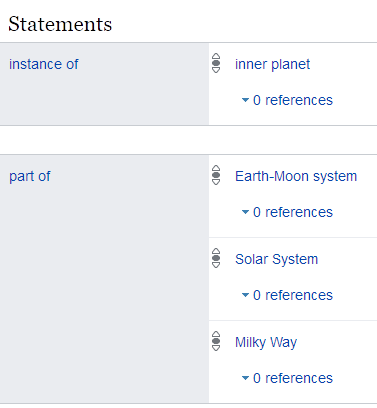
\includegraphics[width=0.7\textwidth]{img/wikidata.png}
\caption{Example of a Wikibase application's use of RDF, here some of the data for "Earth". }
\label{fig:wikidata}
\end{figure}

For the second approach, we installed the Semantic MediaWiki\footnote{\url{https://www.semantic-mediawiki.org}} extension. Together with the Page Forms extension, entering and querying data is very simple. Additionally, it is possible to import external ontologies into the Semantic MediaWiki, as it uses classes and properties to define data. Templates can be defined in order to pre-design Wiki pages so that we only have to submit data instead of writing the same layout repeatedly. With a Semantic MediaWiki, it is currently possible to store the Wiki data in an RDF store. The RDF store in that case acts as a second database where all Wiki data is stored in triples.  

Figure \ref{smwrdf} shows how the components are involved with the use of a Semantic MediaWiki and a triple store. Study data is submitted to the Wiki by the user in the web application. The application then queries data via the RDF store's SPARQL endpoint. This makes it possible to show the user a list of studies they have already submitted. In addition, this easily enables other features such as displaying studies based on keywords or institutions.\\


\subsubsection{MediaWiki Setup}
With the decision to use a Semantic MediaWiki, we next looked at extensions to form our setup. 

Page Forms is an extension that allows us to use templates and forms to fill these templates. That way, users do not have to learn any MediaWiki syntax and we achieve homogeneous study pages. For our scenario, this became especially relevant for file uploads, as will be explained in the next section. \\

Although Wikibase did not turn out to be suitable for us, the RDFIO extension provides a similar functionality in terms of RDF output on Wiki pages. It also comes with a SPARQL endpoint and query editor integrated into the MediaWiki, so users have an additional way to execute SPARQL queries on the data. \\

As choosing the correct version is important for all involved extensions and the MediaWiki itself, Table \ref{tab:mwversion} shows a detailed list of the setup at the time this is written. Apart from the standard products and the mentioned extensions, a database has to be chosen during installation. We chose MariaDB, as it is the standard database used by WikiMedia (cf. \footnote{\url{https://www.mediawiki.org/wiki/Manual:MySQL}} and therefore less likely to cause problems with future updates. Before updating any of the extensions or the MediaWiki itself, compatibility checks have to always be made to keep the installation stable. 

\renewcommand{\arraystretch}{2}%
\begin{table}
\centering
\begin{tabular}{|l|l|}
\hline
\textbf{Product/Extension} & \textbf{Version} \\ \hline
MediaWiki & 1.31.1 \\ \hline
MariaDB & 10.1.36-MariaDB \\ \hline
PHP & 7.2.10 (apache2handler) \\ \hline
Semantic MediaWiki & 3.0.1 \\ \hline
Page Forms & 4.4.2 \\ \hline
RDFIO & v3.0.2 \\ \hline
\end{tabular}
\caption{Installed MediaWiki products and extensions.}
  \label{tab:mwversion}
\end{table}
\begin{figure}
\centering
	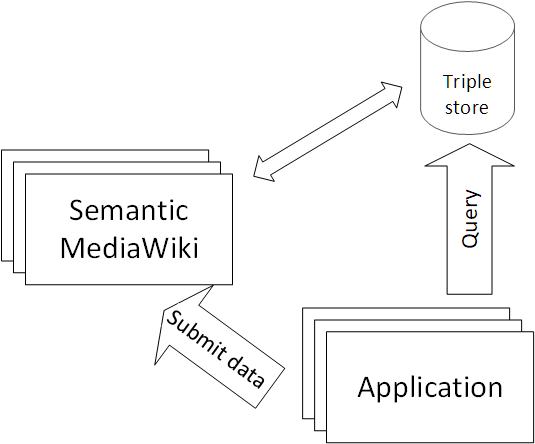
\includegraphics[width=0.8\textwidth]{img/wiki.png}
	\caption{Overview of storage components with a Semantic MediaWiki connected to an RDF store.}
	\label{smwrdf}
\end{figure}	
\subsubsection{Integrating ontologies}
Semantic MediaWiki allows us to import ontologies and use classes and properties as MediaWiki properties. For each ontology, we provide a link and list the properties that we want to use. We then create a new property in the format $Maeo:has property$. Properties are then integrated into page templates by mapping the input data to a property. With the RDFIO extension, the used ontology properties are displayed on the MediaWiki pages that use such a template, as can be seen in the \textit{Facts} box in Figure \ref{fig:template}.


\subsubsection{Interaction between MediaWiki and web application}
After setting up the Semantic MediaWiki, the next step was to submit and retrieve data via the web application. The simplest way to do this is by using the MediaWiki action API. This API already provides the basic functionality needed to create, edit and delete Wiki pages. Several clients for different programming languages are available for an easy integration. We are using the "mediawiki\_api" Ruby gem in our back-end application. We created a simple bot with the rights to edit, create and delete pages to reduce security risks for the API client. Using the bot's credentials, the client asks for a session token and allows for the specified CRUD operations. Since we are using a Semantic MediaWiki, we can create Wiki pages with the templates we have designed for this purpose. The following code fragment demonstrates the simplicity of this template-based setup:
\noindent

\begin{minipage}{0.95\textwidth}
\begin{lstlisting}[frame=single]
{{Study
  |StudyTitle=#{title}
  |ExecutedAtInstitution=#{institution}
  |Country=#{country}
}}
\end{lstlisting}
\end{minipage}

Here, we only have to use values provided by the user (title, institution, country) and insert them into the template skeleton. We use the client to create a Wiki page with the study's ID as the page title for a unique reference URL and only have to transfer this filled out template as the page content. This results in the Wiki page shown in Figure \ref{fig:template}. Changing a template later on, for example adding content or new formatting then only has to be done once. After refreshing all Wiki pages via a php script, the template-using pages are automatically changed according to the new template.\\

\begin{figure}
\centering

	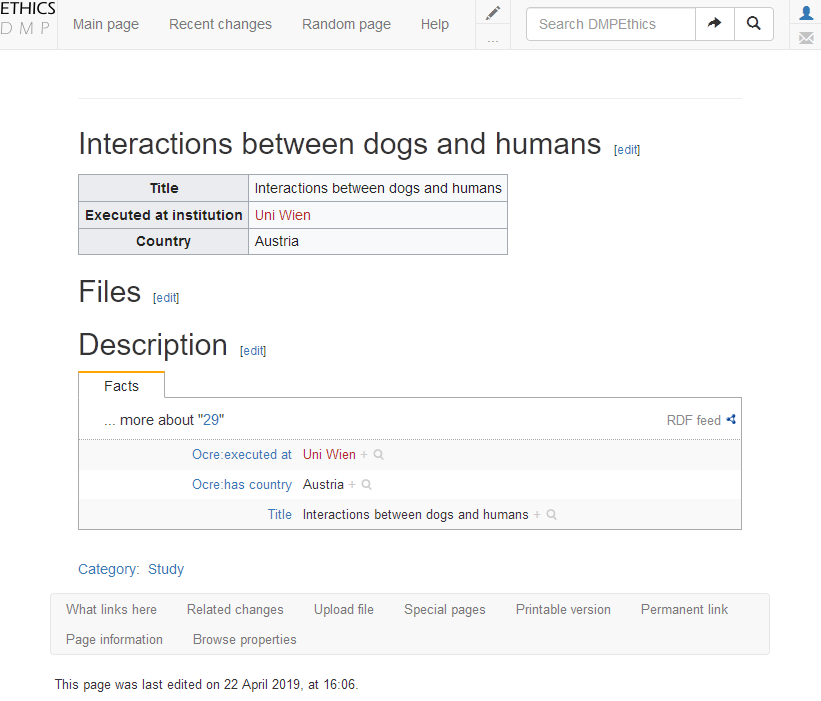
\includegraphics[width=0.8\textwidth]{img/template.png}
	\caption{A Wiki page generated from a simple template.}
	\label{fig:template}
\end{figure}


\subsubsection{PIDs}
One important part of our task was to integrate and create PIDs where needed. We discussed the current state of PIDs in the ethical approval process in Sections 2 and 3 (cf. Figures \ref{pidsnow} and \ref{pidsfuture}). Figure \ref{pidsimpl} shows where we add PIDs during the upload process. PIDs for files are generated in the front-end's checklist feature based on the study ID and a random number, as described earlier. As we store such a PID with each file that is uploaded by the user and associate it with its own property, files are permanently identifiable and searchable by their unique ID.

As we also need a PID for the study itself, we simply use the study's URI. Each study is created as a MediaWiki page by using its unique ID from our PostgreSQL database. We do not repeat IDs, which means that we already have a unique and permanent identifier in the form of \texttt{localhost/wiki/123} (where \texttt{123} is the study's ID).

\begin{figure}
	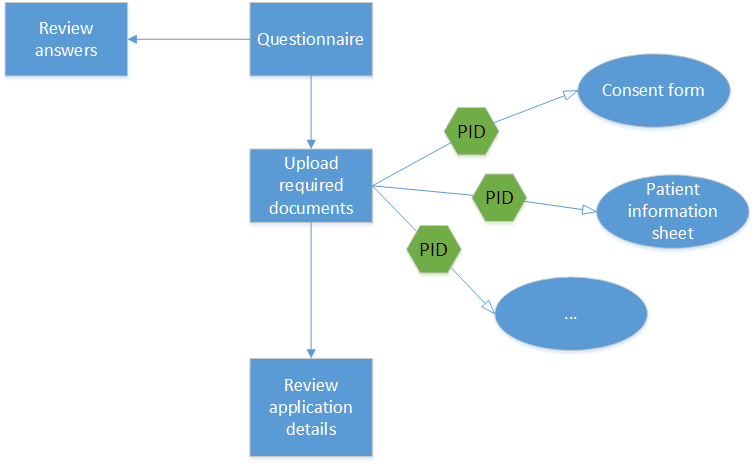
\includegraphics[width=1\textwidth]{img/workflow_1.png}
	\caption{Creation of PIDs during the user's workflow.}
	\label{pidsimpl}
\end{figure}


\subsection{Example walkthrough}

\begin{figure}[H]
\centering
	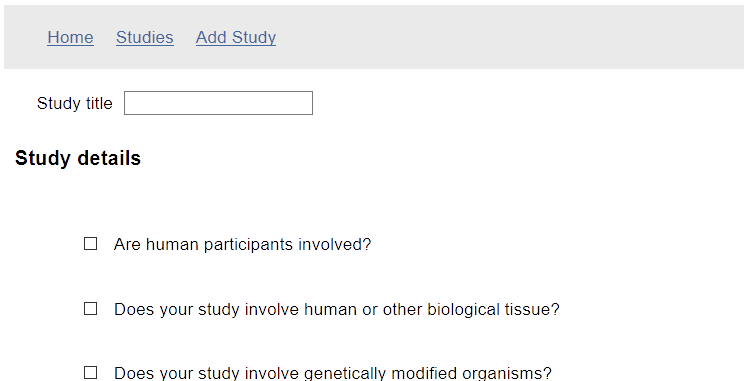
\includegraphics[width=1\textwidth]{img/addstudy.png}
	\caption{The user can add a study by providing a title and filling out a questionnaire.}
	\label{fig:addstudy}
\end{figure}

The user's workflow starts on the web application. In order to create a new study on the application, they first fill in the study title and then go through the questionnaire. (cf. Figure \ref{fig:addstudy})\\

\begin{figure}[H]
\centering
	
\includegraphics[width=1\textwidth]{img/filloutstudy.png}
	\caption{While filling out the questionnaire, the user is shown warnings.}
	\label{fig:filloutstudy}
\end{figure}

As they are answering the questionnaire, warnings and requirements will pop up as infoboxes, as demonstrated in Figure \ref{fig:filloutstudy}. Sub-questions open when their parent question is selected and are visually indicated by their placement relative to their parent question. After submitting the questionnaire, the user is redirected to a list of all studies they have previously created. An example of how this looks to the user can be seen in Figure \ref{fig:studylist}.\\

\begin{figure}[H]
\centering
	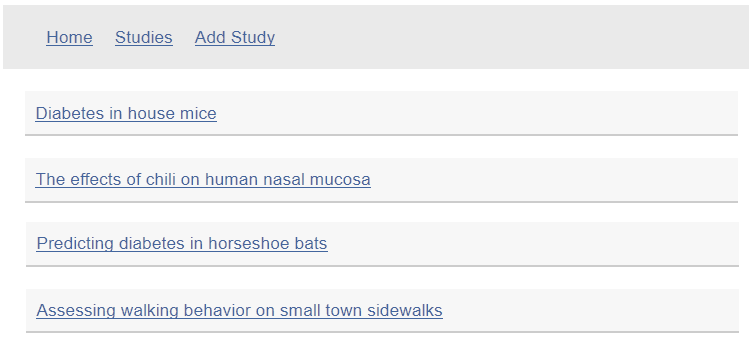
\includegraphics[width=1\textwidth]{img/studylist.png}
	\caption{The user has access to all their submitted studies.}
	\label{fig:studylist}
\end{figure}

This list is also available through the menu. The user can then select a study. A tabbed group of features appears once a study has been selected.\\

\begin{figure}[H]
\centering
	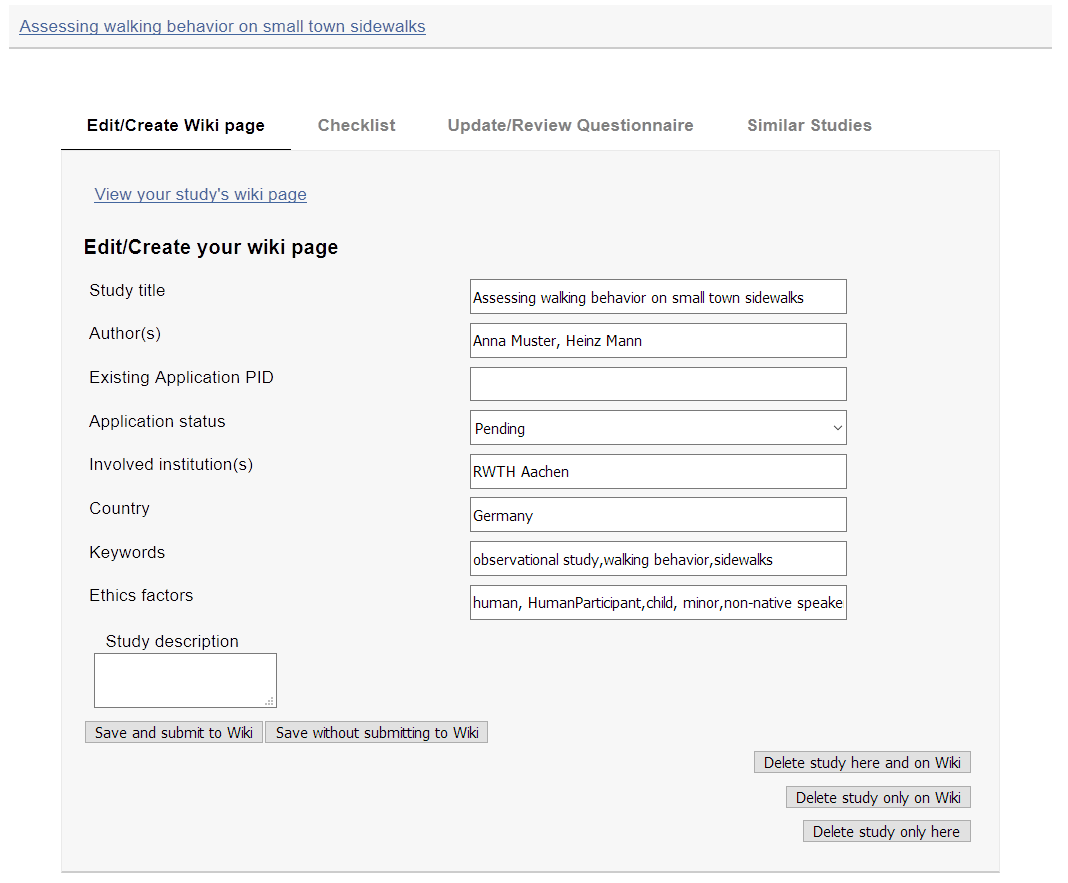
\includegraphics[width=1\textwidth]{img/studysub1.png}
	\caption{A form can be filled with data for the private and/or public databases.}
	\label{fig:studysub1}
\end{figure}

Through the first feature (cf. Figure \ref{fig:studysub1}), the user can add information about their study and save that data to the private PostgreSQL database. They also have the possibility to create and edit their study's Wiki page through this form. We automatically generate a PID after the study has been added. This PID along with ethics factors and the study title is automatically added from the questionnaire input. The ethics factors and the title can still be edited by the user through this form. The user can also delete their study here. For this, they have the option of only deleting the study on the Wiki, only deleting the study from the private database, or deleting the study from both the private database and the Wiki. \\

\begin{figure}[H]
\centering
	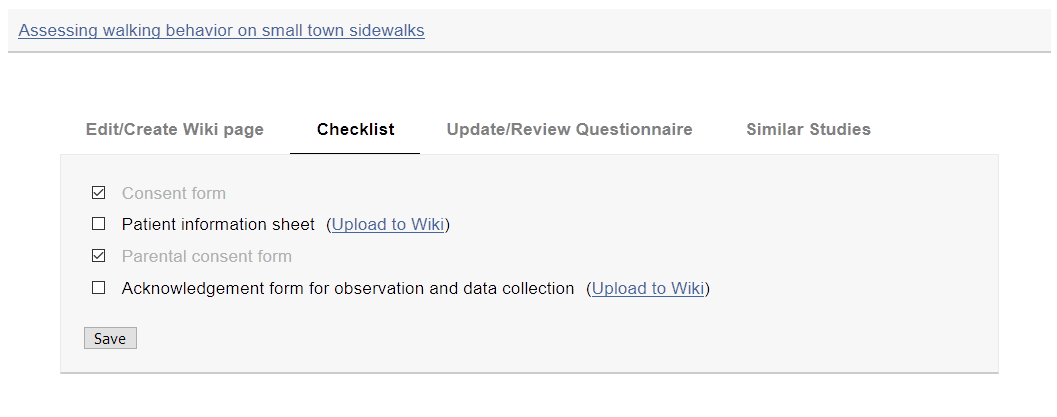
\includegraphics[width=1\textwidth]{img/studysub2.png}
	\caption{A checklist shows the user which documents they should provide. Checklist progress can be saved in the private database.}
	\label{fig:studysub2}
\end{figure}

A checklist with the documents that should be provided with the ethics approval application is automatically generated based on the questionnaire input. This can be seen in Figure \ref{fig:studysub2}. Checklists can be saved in the private database to keep track of the progress. Through a link to a form on the MediaWiki, the user can upload files that will automatically be added to their study's MediaWiki page. For this, the randomly generated file PID and the study PID are sent as hidden form elements, so that the user only has to upload their file.  \\

\begin{figure}[H]
\centering
	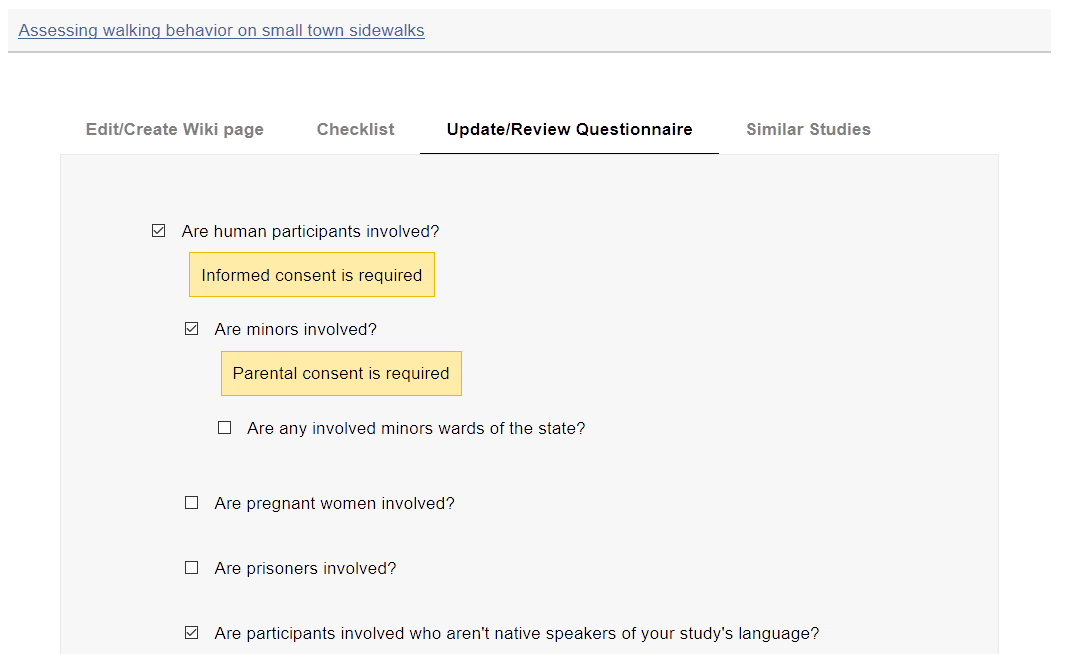
\includegraphics[width=1\textwidth]{img/studysub3.png}
	\caption{The questionnaire can be reviewed and updated.}
	\label{fig:studysub3}
\end{figure}

Through another tab (cf. Figure \ref{fig:studysub3}), the user can review and update their filled out questionnaire. With this feature, they can see all requirements and warnings again in one place.\\

\begin{figure}[H]
\centering
	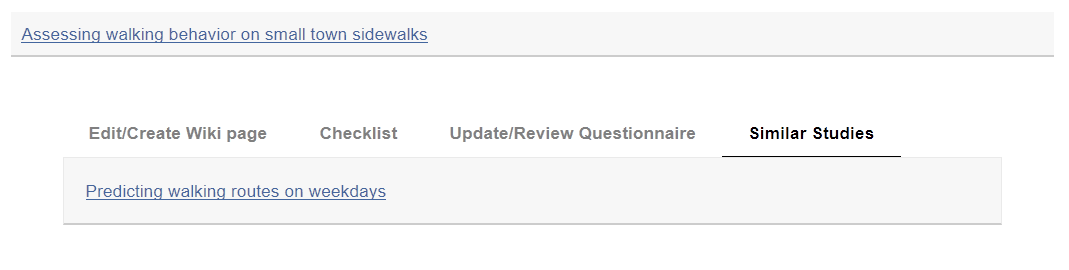
\includegraphics[width=1\textwidth]{img/studysub4.png}
	\caption{Similar studies can be accessed as long as they are public on the Wiki.}
	\label{fig:studysub4}
\end{figure}

Finally, the user has access to the list of similar studies, as shown in Figure \ref{fig:studysub4}. Similar studies are listed as links to that study's MediaWiki page. \\

\begin{figure}[H]
\centering
	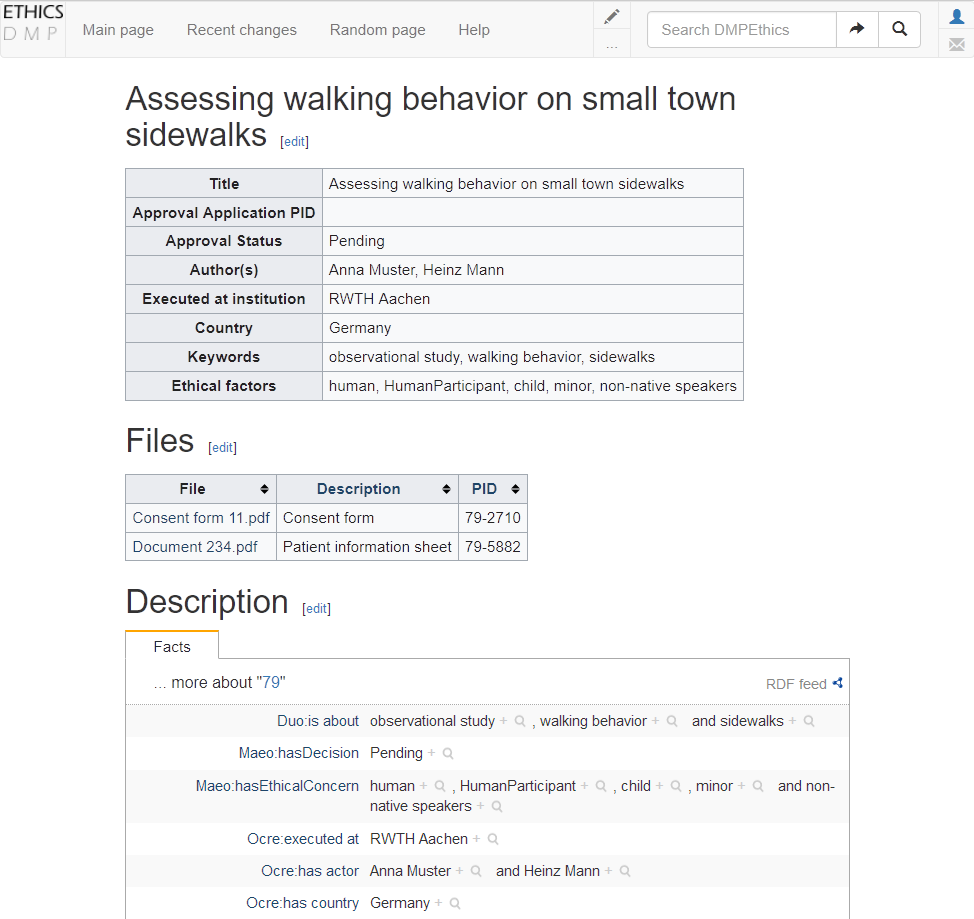
\includegraphics[width=1\textwidth]{img/wikipage.png}
	\caption{Public MediaWiki page showing the submitted study data.}
	\label{fig:wikipage}
\end{figure}

If a user has submitted their study data to the MediaWiki, their data is now publicly accessible. Figure \ref{fig:wikipage} demonstrates how these pages look like. An overview of the submitted study details is shown in text form. Associated files are linked together with a short description and their generated PIDs. At the bottom of the page, the \textit{RDFIO} box allows users to directly search other studies based on the details of this study and shows the used controlled vocabulary. 

\begin{figure}[H]
\centering
	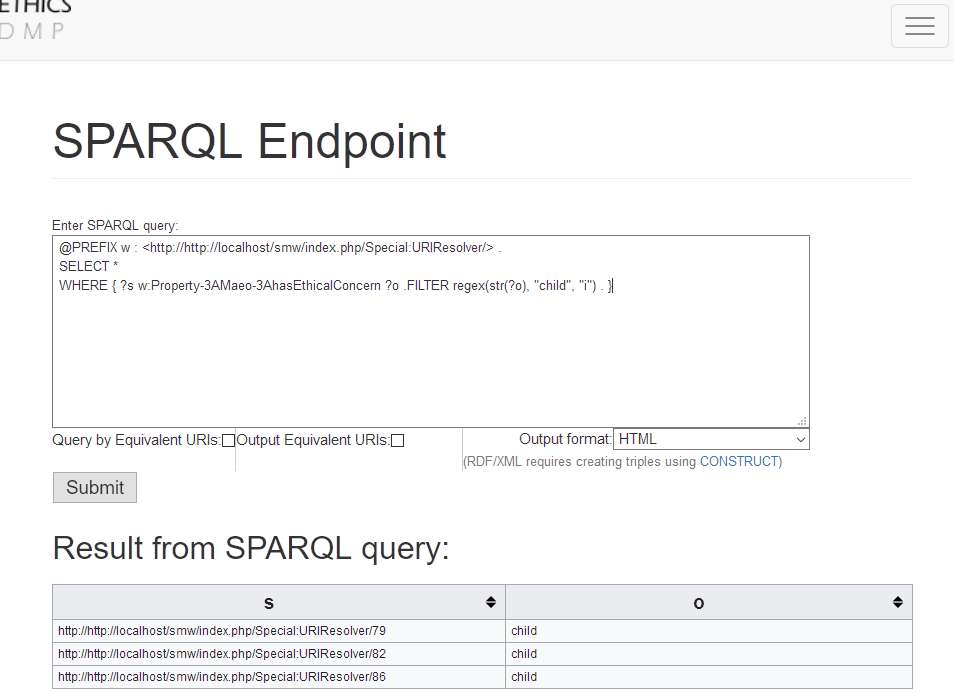
\includegraphics[width=1\textwidth]{img/sparql.png}
	\caption{SPARQL queries can be used to discover studies.}
	\label{fig:sparqlwiki}
\end{figure}

Apart from these small, direct searches, experienced users can also use more elaborate SPARQL queries through the provided endpoint on the MediaWiki. In Figure \ref{fig:sparqlwiki}, a query was executed to find all studies that have listed the involvement of children as a potential ethical issue. As the RDF triplets used in the MediaWiki store the study's URI as the subject, the user can then easily access and explore the listed studies.

\subsection{Evaluation}
To evaluate our concept implementation, we will first evaluate based on the principles for machine-actionable data management plans we have described in Chapter \ref{sec:background}. We will then provide competency questions for SPARQL queries. Finally, we will use a case study to evaluate how an existing study would be entered into the system.

\subsubsection{Evaluating against the principles for machine-actionable Data Management Plans}
We use the earlier given principles (cf. Figure \ref{fig:madmp}, \cite{madmp}) in the context of specifically the management of ethics for an initial evaluation:
\begin{enumerate}
\item \textbf{Integrate DMPs with workflows of all stakeholders:} \\
\textit{Explanation:} Different stakeholders have different workflows. Systems should consider this and integrate interactions that support this, for example with automated actions depending on the stakeholder.  \\
\textit{Our implementation:} We have implemented our application specifically for the author perspective and the research perspective. For ethics committees, we have mainly added the possibility to refer to publicly available data. A deeper integration through interfaces for institutions where committee members can add requirements could be possible, but requires the support of institutions in general.
\item \textbf{Allow automated systems to act on behalf of stakeholders} \\
\textit{Explanation:} Systems should reduce the effort needed to maintain data management plans. This can be achieved through automated data collection, computations, administrative actions and other automated actions.\\
\textit{Our implementation:} As we designed our application as a potential add-on for tools like \textit{DMPTool}, which already collects information in one place and performs other automated actions for stakeholders, we did not need to add much additional functionality. Notifications about when ethics approval expires could be useful, as reminders are usually sent out by the committees individually. We do not however have uniform expiration times across institutions, so such a feature would require the support of institutions and an additional interface for ethics board staff. This could be an idea for future work.
\item \textbf{Make policies for machines, not just people} \\
\textit{Explanation:}  Policies and guidelines concerning collected data should be machine-actionable so that machines can comply to, for example, data sharing rights.  \\
\textit{Our implementation:} From the perspective of ethics, this mainly concerns the data that is collected during the study. We did not implement any data policies, as we only considered documents such as consent forms and other application forms and documents, which are provided by the researchers. For the future, if the application is expanded and integrated with ethics committee workflows, this could be reconsidered again.
\item \textbf{Describe components of data management system for both machines and humans:} \\
\textit{Explanation:} This principle concerns itself with services for data management plans such as data repositories and how they can be found by or recommended to researchers. \\
\textit{Our implementation:} As we did not come across any noticeable services for ethics review processes (apart from the previously discussed \textit{deon} tool for ethics checklists), this is not applicable to us at this time.
\item \textbf{Use PIDs and controlled vocabularies:}  \\
\textit{Explanation:} By identifying data through PIDs, searchability is improved. In contrast to unstructured free-form text, controlled vocabularies reduce noise and provide higher information density. Finding data also becomes easier through this.\\
\textit{Our implementation:} We use ontologies to structure data and have added PIDs to the management of ethics application data and documents.
\item \textbf{Follow a common data model for maDMPs:}  \\
\textit{Explanation:} A common data model is meant to be used for informatoin exchange and as a way to include interoperability.\\
\textit{Our implementation:} As there are currently no applicable data models for our purpose, we cannot implement this at this time. We model user data with JSON and RDF instead of simply saving freetext, which could be helpful for any future data models.
\item \textbf{Make DMPs available for human and machine consumption:}  \\
\textit{Explanation:} DMPs should be available at all times so that they can be accessed throughout the research process by all stakeholders. With structured data and automated update notifications, accessing and managing DMPs is easy for both humans and machines. \\
\textit{Our implementation:} All ethics-related data stored in the application is both available for humans in the form of public storage and for machines by storing data in RDF triplets. As the data is public, it is available for everyone. Choosing to not make data public can be preferred by the researcher. At the moment, we store data that researchers do not want on the MediaWiki in a PostgreSQL database that can restrict data access. Automated notifications of updated data are only available through the MediaWiki's "Watch this page" functionality.
\item \textbf{Support data management evaluation and monitoring:}  \\
\textit{Explanation:} As grant proposals are monitored and evaluated, machine-actionable DMPs need some functionality to support this. Automatic evaluation could be an additional tool next to the evaluation of stakeholders.\\
\textit{Our implementation:} We make monitoring and evaluation easier by storing ethics-related data publicly. This means that all stakeholders can easily access the public data. At the moment, our application does not make enough metadata available to allow stakeholders to evaluate data that has not been made public. Machine-actionability is available through the possibility of checking whether for example consent forms exist on the public MediaWiki. This is possible through MediaWiki queries and SPARQL queries.
\item \textbf{Make DMPs updatable, living, versioned documents:}  \\
\textit{Explanation:} Versioning data management plans creates a record of researchers' input over time. Updating and refining plans should be integrated into the stakeholder workflow.\\
\textit{Our implementation:} The ethics aspects can be updated at all times through the web application and the MediaWiki. The MediaWiki offers versioning through page histories.
\item \textbf{Make DMPs publicly available:}  \\
\textit{Explanation:} Public data management plans help researchers of a single study collaborate and allows stakeholders to easily pull data from multiple plans. Public data also enables findability and accessibility.\\
\textit{Our implementation:} The ethics part of DMPs is publicly available via the Semantic MediaWiki.
\end{enumerate}

\subsubsection{Competency questions}
We have previously listed features and their feasibility in Table \ref{tab:featuresa}. We have implemented these features as described.
To demonstrate the usability of the public data storage, we compiled a list of competency questions. Via the implemented SPARQL endpoint, these questions can be answered successfully:

\begin{itemize}
    \item For a given ethical concern (e.g. prisoners), find the studies that contain it.
    \item For a given PID, find the pages or files associated with it.
    \item For a given topic or keyword, find the ethical concerns related to it in existing studies.
    \item For a given ethical concern, find the files associated with it.
    \item For a given institution, show the success of applications given an ethical concern.
    \item For a given document type (e.g. consent form), show all files of that type.
\end{itemize}

We use a controlled vocabulary and machine-readable formats for storing ethics data through our ontology, which makes these queries possible. By fulfilling the criteria for findability of the available data, our application is suitable for research.

\subsubsection{Case study}
For this case study, we will use the data available in \cite{casestudy}, which was also used as an example in the introduction. This data is available under the Creative Commons Attribution Share Alike 4.0 license \footnote{\url{https://creativecommons.org/licenses/by-sa/4.0/}}, which allows us to share and reuse.\footnote{\url{https://data.qdr.syr.edu/dataset.xhtml?persistentId=doi:10.5064/F6MS3QNV}}

We start by using the questionnaire to enter data. The study involved human participants that do not appear to be described as vulnerable as far the public information for this study shows. The authors requested approval from the University of Texas at Austin, but the interviews conducted tool place in Latin America. Figures \ref{fig:1} and \ref{fig:2} show the filled out questionnaire according to this information.
\begin{figure}[H]
\centering
	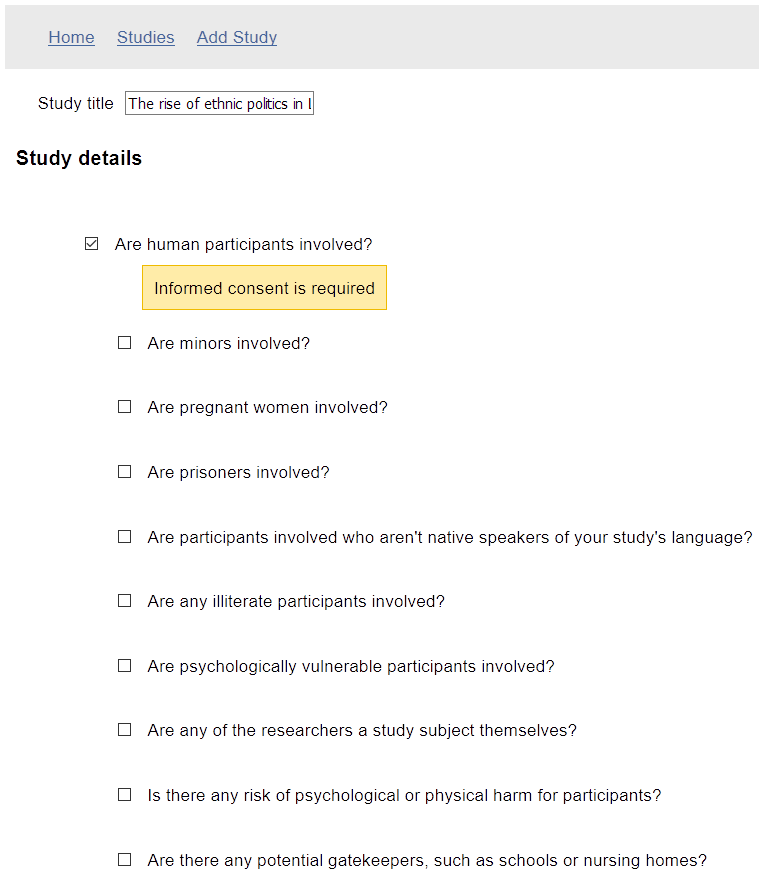
\includegraphics[width=1\textwidth]{img/1.png}
		\caption{Case study: Questionnaire, pt. 1}

	\label{fig:1}
\end{figure}
\begin{figure}[H]
\centering

	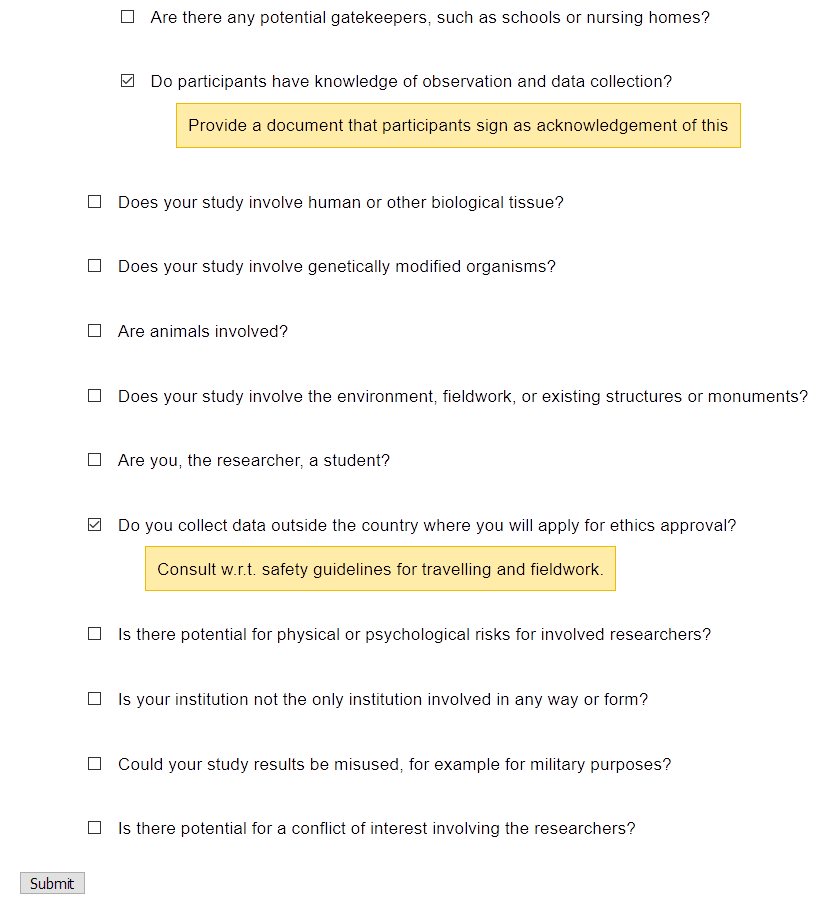
\includegraphics[width=1\textwidth]{img/2.png}
	\caption{Case study: Questionnaire, pt.2}
	\label{fig:2}
\end{figure}

Our application then identified the requirements shown in Figure \ref{fig:3}. The study in reality only had to submit a consent form in order to successfully gain approval. This consent form informed the participants of potential risks and their compensation (in this case none). The information given does combine a consent form with the acknowledgement for data collection. This example shows that approval requirements can be different from institution to institution, and that the given requirements may therefore not match the actual requirements. A requirements database that pulls requirements depending on a selected institution could solve this, but collecting this data would require much effort. If ethics committees are open to this, participating institutions could simply enter their requirements instead.
\begin{figure}[H]
\centering
	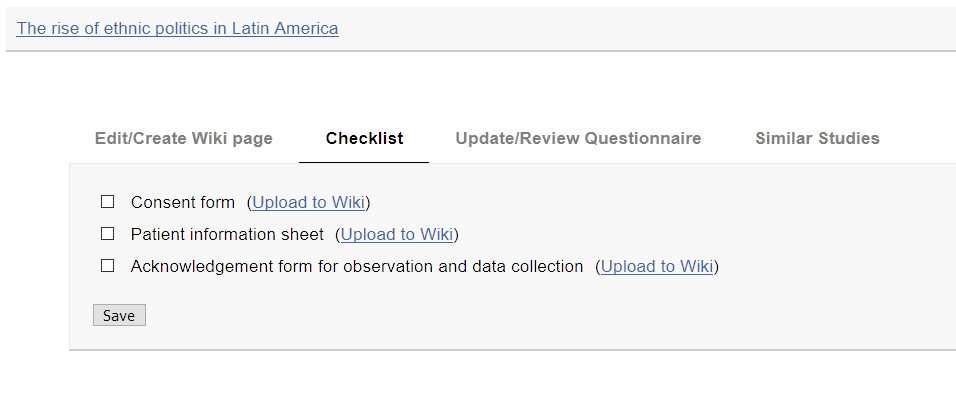
\includegraphics[width=1\textwidth]{img/3.png}
	\caption{Case study: Requirements}
	\label{fig:3}
\end{figure}

\begin{figure}[H]
\centering
	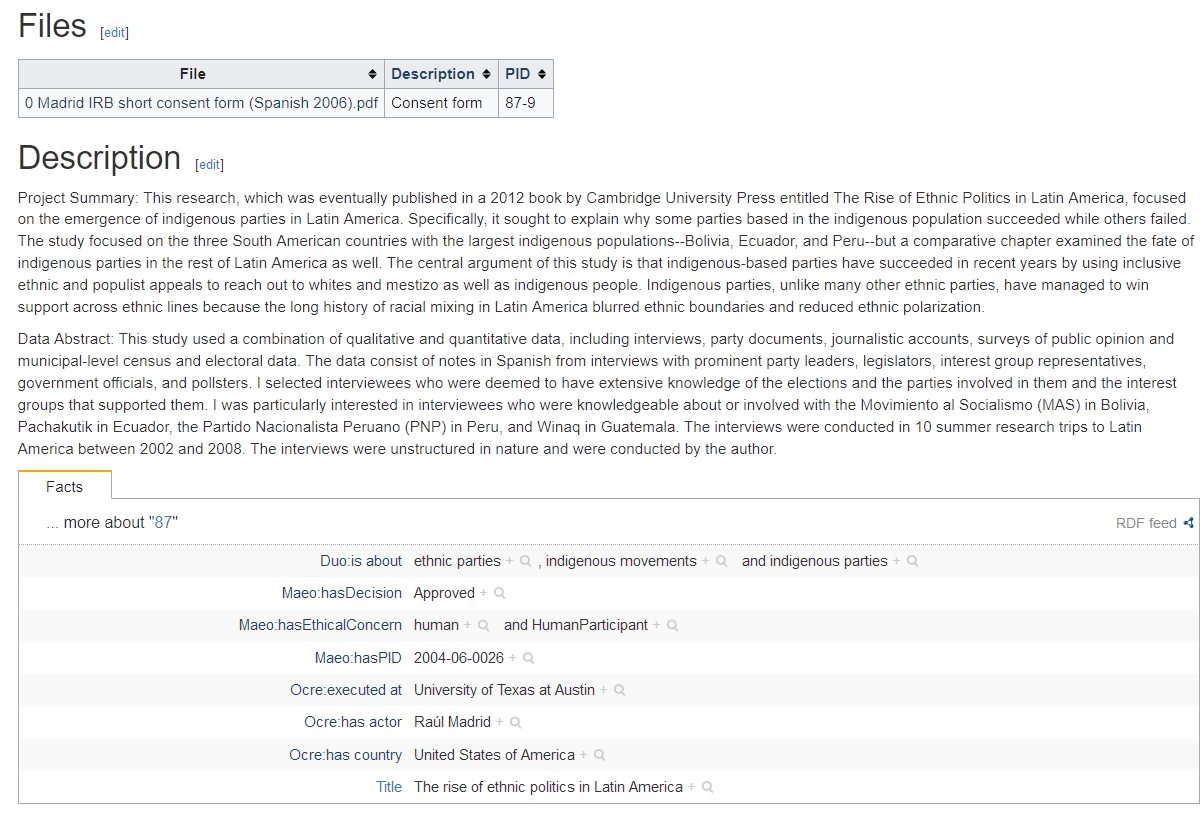
\includegraphics[width=1\textwidth]{img/4.png}
	\caption{Case study: Wiki page}
	\label{fig:4}
\end{figure}

Figure \ref{fig:4} shows the data as available in the Semantic MediaWiki after submitting it through our web application. When compared to the current data repository for the study and its documents\footnote{\url{https://data.qdr.syr.edu/dataset.xhtml?persistentId=doi:10.5064/F6MS3QNV}}, our solution provides direct links to related data and easy searchability from the submitted data. As not all information may be made public (as seen in the access-restricted files in the original repository), adding metadata as in the given repository would be beneficial.

We have shown that although the listed requirements were more than actually needed to gain ethical approval, our application is capable of handling existing data and making it findable and accessible. 

\subsection{Summary}
In this chapter, we have described our implementation process and the resulting application. We listed potential features for different stakeholders that we had identified after the analysis phase and discussed whether an implementation would be feasible for each feature. Based on the feature list and existing tools such as \textit{DMPTool}, we designed the architecture for our implementation, which consists of a \textit{Ruby on Rails} API application and a \textit{Vue.js} frontend. The user's workflow was given as a guideline before going into detail on how we implemented the individual features. An investigation of the ideal public data storage was described as well. We have integrated PIDs and the controlled vocabulary we have provided in our ontology into the management of ethics data wherever it made sense. Finally, we have looked at how our application adheres to the guiding principles for machine-actionable data management plans. We also provided a list of questions that we used to test the competency of our data storage through SPARQL queries. Through a case study we examined the potential and  the drawbacks of our concept. The benefit of future expansion through a better integration in the ethics approval processes with support from interested institutions and the addition of metadata became clear.

\newpage

\section{Conclusion}
\label{sec:conclusion}

\subsection{Summary}
After going into the background of machine-actionable data management plans and FAIRness, we have discussed related work relevant to our topic. An extensive analysis phase was conducted before formalizing the gained knowledge. Ethics approval processes were shown to often be a significant hurdle for research teams. Special cases that are not reflected by most ethics committee guidelines and a lack of ethics knowledge can lead to the rejection of applications. Administrative errors such as missing hand-ins and the complexity of dealing with multiple institutions for a single study can set back studies by months. Secondary research faces other issues as ethics-related documents are rarely available after approval decisions have been finalized. Investigating the ethical considerations behind certain studies as study participants can be hard for the same reason. By identifying these problems, we gained a basis for designing solutions that help researchers. We have presented a pattern language that can be used for further work and implementations. Within a given context, our patterns sketch out possible solutions and things to consider. An ontology that integrates existing ontologies into one that is focused on the ethics approval process provides the necessary controlled vocabulary for machine-actionability. 

Based on our pattern language and the analyzed common problems in ethics research, we have realized a concept application that aims to solve as many of these issues as possible. Researchers have access to an application that allows them to manage their ethics-related data. Through the application's questionnaire, we can identify the most common ethical issues for the study scenarios we derived from our previous analysis of the ethics approval process. With this information, we can provide the user with a checklist and warnings that signal potential ethical problems to the user. A public data store in the form of a Semantic MediaWiki combined with an RDF store adds findability and accessibility to a machine-actionable ethics workflow. Documents such as consent forms can there be accessed by interested users and are permanently identifiable through PIDs. With the implemented extensions, both experienced and inexperienced users can conduct searches. SPARQL queries serve as the main solution to find study data.

We have overall attempted to add machine-actionability to ethics approval workflows that have previously been closed off from the public and are often opaque. Our formalization of the process and our concept implementation are open for further research.

\subsection{Outlook}
Although we can try to make the ethics process as machine-actionable as possible, the question whether ethics committees are open for change remains. As documents and decisions are kept in private storage and not always in digital format, opening the process up for outsider insight can be a drastic change. Already existing studies may not have the relevant data such as ethics application PIDs and consent forms available anymore, especially when ethics applications are only kept in storage for a limited amount of time. For this reason, it is not realistic to expect all previously existing ethics data to become publicly available. Therefore, the focus should lie on improving the situation for future studies before attempting to make previous ethics application processes public.

Future improvements can be implemented both for the MediaWiki storage solution and the web application. As the MediaWiki develops, structured storage will likely be integrated better instead of requiring additional extensions or external RDF stores. Although RDF-based extensions are available, they require additional effort in maintaining and may become inactive and unsupported over time. A good structured data store in MediaWikis could open up the possibility of reliably executing SPARQL queries on RDF data from outside the MediaWiki. Queries could then be executed from the separate web application.

In our implementation efforts, we have mainly focused on PIDs and structuring study data as well as integrating controlled vocabulary. In addition to this, metadata files could be generated for each study, as is recommended in the FAIR principles. Both administrative information such as the upload date for forms and files and descriptive metadata could be collected from the submitted data and structured and displayed in a meaningful and helpful way. The possibilities of making only the metadata, or both metadata and data could also be explored.

As research on making ethics approval processes machine-actionable and more transparent is ongoing and current, this topic can overall be explored further, and future efforts can be made for additional stakeholders in the ethics process. 

\newpage
\clearpage
\addcontentsline{toc}{section}{References}
\bibliography{ethicsapprovalworkflows}
\bibliographystyle{plainurl}
\newpage
\addcontentsline{toc}{section}{List of Figures}
\listoffigures
\newpage
\appendix
%\addtocontents{toc}{\protect\contentsline{chapter}{Appendix:}{}}
\section{Appendix: Ontology}
All entities and properties from external ontologies are marked with that ontology's shorthand. As the DSAP ontology is not available for consultation anymore, we will note here that the \textit{Action} and \textit{Actor} classes and subclasses have been inspired by that ontology.
\subsection*{Classes}
 
 \begin{itemize}
 \item Action
 	\begin{itemize}
 		\item ApprovalAction
 			\begin{itemize}
 				\item ApprovalDecision
 				\item ApprovalExtension
 			\end{itemize}
 		\item DataObjectAction
 			\begin{itemize}
 				\item AccessDataObject
 				\item DeleteDataObject
 				\item ReuseDataObject
 				\item StoreDataObject
 				\item UseDataObject
 			\end{itemize}
 	\end{itemize}
 \item Actor
 	\begin{itemize}
 		\item DataCollector (AGRO)
 		 	\begin{itemize}
 		 		\item OutsidePersonnel
 		 		\item Researcher 
 			\end{itemize}
 		\item EthicsCommitteeMember (DICOM)
 	\end{itemize}
 \item data item (IAO)
 \item DataStorage(NCIt)
 \item Date
 \item EthicsApproval
  	\begin{itemize}
  		\item ethics approval required (DUO)
  		\item EthicsApprovalRestriction
 	\end{itemize}
 \item EthicsApprovalApplication
  	\begin{itemize}
  		\item Document (NCIt)
  			 	\begin{itemize}
  			 		\item informed consent form (IAO)
 				\end{itemize}
 		\item Form
 			 	\begin{itemize}
 			 		\item ApplicantInformation (NCIt)
 			 		\item DataStorageInformation
 			 		\item EthicalConsideration
 			 		\item StudyInformation
 				\end{itemize}
 	\end{itemize}
 \item Informed consent
  	\begin{itemize}
  		\item ParentalConsent
 	\end{itemize}
 \item Institution (NCIt)
 	 	\begin{itemize}
 	 		\item Ethics approval process (IAO)
 	 		\item EthicsCommittee (NCIt)
 		\end{itemize}
 \item PID
 \item Study (IAO)
 	 	\begin{itemize}
 	 		\item Result
 	 		\item Study design (IAO)
 	\end{itemize}
 \item StudyObject
 	\begin{itemize}
 	\item Animal (STY)
 	 	\begin{itemize}
 	 	\item Invertebrate
 	 	\item Vertrebrate (STY)
 	\end{itemize}
 	\item EthicalConcern
 	\item GMO (NCIt)
 	\item HumanParticipant
 	 	\begin{itemize}
 	 	\item Minor
 	 	\item PregnantWoman
 	 	\item Prisoner (ICO)
 	 	\item VulnerableParticipant
 	\end{itemize}
 	\item InanimateObject
 	 	\begin{itemize}
 	 	\item CulturalHeritage
 	\end{itemize}
 	\item Organic\_natural\_material
 	\end{itemize}
 \end{itemize}
    
    \subsection*{Properties}
    
\begin{itemize}
    \item executed at (OCRE)
    \item has actor (OCRE)
    \item has country (OCRE)
    \item is restricted to (DUO)
    \item member of (DUO)
    \item requires consent
    \item requires parental consent
    \item associatedWith
    \item collectedFrom
    \item concerningActor
    \item concerningDataObjects
    \item conducts
    \item giveConsent
    \item grantsApproval
    \item hasApprovalDate
    \item hasApprovalProcess
    \item hasCommittee
    \item hasDate
    \item hasDecision
    \item hasDeletionDate
    \item hasEthicalConcern
    \item hasExpirationDate
    \item hasFileType
    \item hasForm
    \item hasFormSection
    \item hasPID
    \item hasResult
    \item hasSpecification
   \item  ofStudy
    \item requires
    \item stores
\end{itemize}



\newpage
\section{Appendix: Questions}
\begin{itemize}
\item Are human participants involved?
\item Are minors involved?
\item Are any involved minors wards of the state?
\item Are pregnant women involved?
\item Are prisoners involved?
\item Are participants involved who aren't native speakers of your study's language?
\item Are any illiterate participants involved?
\item Are psychologically vulnerable participants involved?
\item Are any of the researchers a study subject themselves?
\item Is there any risk of psychological or physical harm for participants?
\item Are there any potential gatekeepers, such as schools or nursing homes?
\item Do participants have knowledge of observation and data collection?
\item Does your study involve human or other biological tissue?
\item Does your study involve genetically modified organisms?
\item Are animals involved?
\item Are the animals vertrebrates?
\item Are the animals non-vertrebrates, and not cephalopods?
\item Are the animals cephalopods?
\item Does your study involve the environment, fieldwork, or existing structures or monuments?
\item Could there be potential risk for the environment?
\item Does your study involve work on existing monuments?
\item Will your study take place on private property?
\item Are you, the researcher, a student?
\item Do you collect data outside the country where you will apply for ethics approval?
\item Is there potential for physical or psychological risks for involved researchers?
\item Is your institution not the only institution involved in any way or form?
\item Could your study results be misused, for example for military purposes?
\item Is there potential for a conflict of interest involving the researchers?
\end{itemize}
\end{document}